%% load necessary packages
\documentclass[paper=a4, fontsize=11pt,parskip=half,headings=small]{scrartcl}
\usepackage{check-short}
\usepackage{overpic}
\usepackage{multirow}


%% set author information etc
\title{A Validity Study for Perfusion Measurements in the Capillary System}
\author{Constantin Heck, Erik A. Hanson, \\ Arvid Lundervold, Jan Modersitzki, Alexandre Malyshev, Erlend Hodneland \\ (random order)}
\date{\today}


%% define some local commands
\newcommand{\Qso}{Q_{\mathrm{so}}}
\newcommand{\Qsi}{Q_{\mathrm{si}}}
\newcommand{\ca}{c_\mathrm{a}}
\newcommand{\CBV}{\mathrm{CBV}}
\newcommand{\MTT}{\mathrm{MTT}}
\newcommand{\cout}{c_{\mathrm{v}}}
\newcommand{\Pa}{P_{\mathrm{a}}}
\newcommand{\Pout}{P_{\mathrm{v}}}


%define SI-units, since we want to be able to easily change them
\newcommand{\siFmm}{\milli\meter\cubed\per\second}
\newcommand{\siQmm}{\milli\meter\cubed\per\second\per\milli\meter\cubed}
\newcommand{\siPml}{\milli\litre\per\second\per100\milli\litre}
\newcommand{\siq}{\milli\meter\cubed\per\second\per\milli\meter\squared}
\newcommand{\siml}{\milli\litre}
\newcommand{\siphimm}{\milli\meter\cubed\per\milli\meter\cubed}
\newcommand{\siJ}{\milli\mol\per\second\per\milli\meter\squared}
\newcommand{\siphi}{\milli\meter\cubed\per\milli\meter\cubed}
\newcommand{\sirho}{\milli\gram\per\milli\meter\cubed}
\newcommand{\siQtilde}{\milli\gram\per\second\per\milli\meter\cubed}
\newcommand{\sic}{\milli\mol\per\milli\meter\cubed}
\newcommand{\simm}{\milli\meter\cubed}

%\newcommand{\siP}{\cubic\milli\meter\per\second\per\cubic\milli\meter}
%\newcommand{\siP}{\milli\meter\cubed\per\second}
%\newcommand{\siPml}{\milli\litre\per\second}
%\newcommand{\siQtilde}{\milli\gram\per\second\per\milli\meter\cubed}
%\newcommand{\siQ}{\milli\meter\cubed\per\second\per\milli\meter\cubed}
%\newcommand{\sirho}{\milli\gram\per\milli\meter\cubed}
%\newcommand{\sic}{\milli\mol\per\milli\meter\cubed}
%\newcommand{\siPn}{\milli\litre\per\minute\per100\milli\litre}
%\newcommand{\simm}{\milli\meter\cubed}


%define misc commands
\newcommand{\missingsource}{\textcolor{red}{[?]}}

%--------------------------------------------------------------------------------------------
%--------------------------------------------------------------------------------------------
% Here begins the document, remove "draft" option in document class to include images
%--------------------------------------------------------------------------------------------
%--------------------------------------------------------------------------------------------
\begin{document}
	%--------------------------------------------------
	% Title Page=
	%--------------------------------------------------
	\maketitle
%	\tableofcontents

	
	%--------------------------------------------------
	%--------------------------------------------------
	% Section: Introduction
	%--------------------------------------------------
	%--------------------------------------------------
	\section{Introduction}
	
	Quantitative medical measurements based on tracer kinetic models is an important field both in research and in clinical practice \cite{zierler62,axel80,zierler00}. 
	In the present work, we focus on mathematical models for estimating blood perfusion in the brain (cerebral blood flow, CBF) from contrast-enhanced dynamic MR 	imaging data. Still, the theory on tracer dynamics covered here will also be of relevance in general perfusion studies using other image modalities.

	While hardware limitations in medical imaging for decades have confined studies to only handle larger tissue regions or full organs, modern MR technology and voxel based analysis give rise to aspirations about detailed perfusion maps with millimeter precision.  
	Examples of estimated parameter maps are found in i.e. \missingsource. The quantitative perfusion maps (and other parameter maps arising from tracer kinetic modelling) can be combined with anatomical information, and the maps have proven to be of particular value in e.g. stroke studies for localization of trauma \missingsource. 
	Among the physiological parameters obtainable from tracer kinetic models, CBF has proven to be particularly difficult to reliably describe on a voxel-basis \cite{kudo10}.  
	In several studies, CBF is therefore only reported in relative values and the corresponding parameter maps are mostly used in a qualitative manner \cite{calamante99}.
	The methodological limitations in perfusion estimations are caused both by issues in the numerical implementation, but also by over-simplified dynamic models.  
	It is has been widely studied how delay and dispersion of the contrast bolus between the AIF and the voxel as well as assumptions about directional flow \cite{thacker03,sourbron14} effects the perfusion estimation. 
	In \cite{sourbron14}, a mathematical theory for voxelwise perfusion is introduced and proposed as an alternative to the classical ROI (region of interest) based models for perfusion. 
	In this work, we will use some of the same physical concepts introduced for voxelwise perfusion, and relate them to the classical ROI based perfusion models.  
	We will further discuss limitations of classical models applied voxel wise, and study their validity in an unstructured flow field.
	The pharmacokinetic models, and how they behave under different ROI/voxel sizes and shapes, are analyzed mathematically and evaluated within a synthetic flow field.  
	A mathematical framework is also derived, in which the medical notion of perfusion can be understood in a physically more precise manner.

	Evaluation of perfusion models using a synthetic flow field is also performed in i.e. \cite{calamante03}. 
	Here, the synthetic model is based on solution of Navier-Stokes equations within the arterial system and the effect of dispersion is studied.  
	In the present work, we model the contrast agent (CA) propagation through a small section of the capillary system. 
	Both these approaches require several clarifying assumptions on flux and propagation. 
	In pharmacokinetic analysis it is often assumed that each ROI (voxel) is an autonomous system that can be modeled by standard pharmacokinetic theory \missingsource. 
	As in \cite{calamante03}, we study CA propagation through a larger area with a highly developed capillary/arterial system and thereby consider a range of connected problems where each voxel can be regarded as an inlet for the surrounding voxels.  
This more accurately mimics the nature of blood flow in the tissue.  
	Unlike Calamante et al. \cite{calamante03} we also distinguish between scalar perfusion maps, describing flow normalized over a volume, and the physical, vector valued flux field, describing flow normalized over a surface area. 


	The rest of this paper is arranged as follows: In Section \ref{sec:classical}, we outline classical methods for perfusion estimation and discuss two widespread solution methods. 
	In Section \ref{sec:synthetic} we describe how a synthetic flow field in the capillary system can be modelled using simple models valid within porous media. 
	We also discuss mathematical similarities between the flow field models and the classical theory outlined in Section \ref{sec:classical}. 
	\textcolor{red}{Some missing sections here?}
	In Section \ref{sec:results} we evaluate the performance of classical models by applying them to the synthetic flow field. 
	The results and concluding remarks are summarized in Section \ref{sec:conclusion}.
	
	
	
	%--------------------------------------------------
	%--------------------------------------------------
	% Section: Classical models
	%--------------------------------------------------
	%--------------------------------------------------
	\section{Classical Models for perfusion} \label{sec:classical}

	Classical theory for pharmacokinetic modelling is used to recover CBF, cerebral blood volume (CBV), as well as mean transit times (MTT) from data displaying propagation of a contrast agent through the tissue.
	The so-called deconvolution model (DM) is used in vast amount of publications \cite{ostergaard96,abels10,straka10,bivard13,sourbron13}.
	Restoration of CBF yields reasonable results \missingsource, however validation is a problem as ground-truth CBF is hard to determine.
	Validation of novel implementations is usually done in the so-called \emph{inverse crime} setting. 
	This means that the forward model used to generate data and the backward model to reconstruct parameters are similar, if not identical. However, the physical validity of the model can still be questionable.
	Another model for perfusion which has been used for restoring CBF and MTT is the so-called maximum slope model (MS) \cite{miles91,klotz99}.
	The maximum slope model only considers early time points and it has been shown to exhibit advantages over the deconvolution model especially if uptake curves are degraded in the late phase \cite{abels10}.
	However, since it relies on point-wise estimates, application to real data is nevertheless difficult and prone to noisy measurements.
	Also, the maximum slope model inherently assumes that no outflow takes place when the AIF peaks (see Sec. \ref{sec:ms}).
	This assumption is questionable for arbitrary, maybe pathological tissue with possibly prolonged MTT \missingsource.
	
		
	Following \cite{sourbron13}, we now briefly present the common theoretical basis of the two models.
	Let $\Omega_i$ be a control volume with one inlet and one outlet and let $C(t)$ denote the average CA concentration within $\Omega_i$ at timepoint $t$.
	Let us furthermore assume linearity and stationarity \textcolor{red}{What is linear and what is stationary?} of CA in- and outflux with proportionality constants $\Pa, \Pout$  [\si{\siQmm}].
	These assumptions lead to the differential equation $C'(t) = \Pa\ca(t) - \Pout\cout(t)$, reflecting mass balance of the tracer. 
	Here $\ca,\cout$ are the CA concentrations at the inlet and outlet of $\Omega_i$.
	Assuming incompressibility of flow leads to $\Pa = \Pout$ and hence we obtain the general form
	\begin{equation}
		C'(t) = \Pa\left(\ca(t) - \cout(t)\right).
		\label{eq:classicgeneral}
	\end{equation}
	In the next step, the deconvolution model and the maximum slope model are diverging based on different assumptions.

	%----------------------------------------------------------
	% Subsection: The Convolution Model: Theory and Implementation
	%----------------------------------------------------------	
	\subsection{The Convolution Model: Theory and Implementation}\label{sec:conv}
	
	For the deconvolution model it is assumed that there is a probability distribution of transit times $h(t)$ through $\Omega_i$. 
	This leads to
	\begin{equation}
		\cout(t) = (h*\ca)(t) := \int_0^t \ca(s) h(t-s) \diffint s.
	\end{equation}
	Combining this with \eqref{eq:classicgeneral} yields $C'(t) = \Pa\ca(t)-\Pa (h*\ca)(t)$.
	Integrating this equation and using basic properties of the convolution one obtains
	\begin{equation}
		C(t) = (I*\ca)(t).
		\label{eq:conv}
	\end{equation}
	Here the \emph{impuls-response function} $I$ is defined as $I(t) := \Pa(1-\int_0^t h(s) \diffint s)$, and it fulfills the following properties:
	\begin{itemize}
		\item $I(0) = \Pa$,
		\item $I$ is monotonously decreasing,
		\item $I\ge 0$.		
	\end{itemize}
	The task of identifying $I(t)$ given a tissue curve $C(t)$ and an arterial input function $\ca(t)$ is a deconvolution problem.
	If $I(t)$ is recovered, $\Pa$ can subsequently be estimated as $\Pa = \max_{t} I(t)$.
	There are several methods to perform the deconvolution.
	A standard approach using Fourier-based algorithms is sensitive to the presence of noise \cite{ostergaard96,wirestam00}.
	Another class of deconvolution algorithms gaining increasing attention are based on Bayesian modeling \cite{boutelier12,mouridsen06}.
	Recent evaluations are showing good performance \cite{sasaki13}, however the numerical handling is still difficult since complex and error-prone numerical integration has to be performed.
	The most popular among deconvolution algorithms are based on singular value decomposition (SVD) \cite{ostergaard96}.
	These algorithms have shown to be robust for a reasonable noise level.
	Also, they can be easily adapted to be robust against delays in tracer arrival using block-circular structures (bSVD cf. \cite{wu03}).
	In order to identify the impuls-response function $I(t)$ from simulated data, we hence decided to use the bSVD model as proposed in \cite{wu03}.

	%----------------------------------------------------------
	% Subsection: A Second Digital Phantom For Validation
	%----------------------------------------------------------	
%	\subsection{The Convolution Model for a Well-Mixed Compartment \textcolor{red}{Haven't we used this assumption earlier?}} \label{sec:comp}

	If we make the assumption of $\Omega_i$ as a well-mixed compartment where $C(t) = CBV\cout(t)$ for a $0 \le CBV \le 1$, equation \eqref{eq:classicgeneral} reduces to the initial value problem
	\begin{align*}
		(CBV \cout)' &= \Pa \ca - \Pa \cout, \\
		\cout(0)&=0,
	\end{align*}
	where we also assume no tracer within the compartment for $t = 0$. 
	
	Letting $\MTT:=\Pa/CBV$ yields the solution
	\begin{equation}
		C(t) = \Pa \int_0^t e^{-(t-s)/\MTT}\ca(s)\diffint s
		\label{eq:classicalperf}
	\end{equation}
	with residue function $R(t)=e^{-t/\MTT}$. 

	
	
	
	%----------------------------------------------------------
	% Subsection: The Maximum Slope Model
	%----------------------------------------------------------
	\subsection{The Maximum Slope Model}\label{sec:ms}	
	In the MS model it is assumed that at the beginning when $\ca$ peaks, only a negligible amount of CA is leaving the system (cf. \cite{klotz99}).
	For this time interval equation \eqref{eq:classicgeneral} reduces to 
	\begin{equation}
		C'(t) = \Pa\ca(t),
	\end{equation}
	in case one can see that if $\ca$ has a maximum, also $C'$ must have a maximum since stationarity in $\Pa$ is assumed.
	Hence, it holds that
	\begin{equation}\label{eq:MS}
		\Pa = \frac{\max_{t}C'(t)}{\max_{t}\ca(t)}.
	\end{equation}
	
	
	
	%--------------------------------------------------
	%--------------------------------------------------
	% Section: The synthetic model
	%--------------------------------------------------
	%--------------------------------------------------	
	\section{A Synthetic Model for Capillary Perfusion}\label{sec:synthetic}
	
	Structurally, the model-assumptions for both classical methods presented in Section \ref{sec:classical} are similar.
	The validity of both methods rely on a ROI having only one inlet and one outlet, and that the CA concentration is well mixed within the entire compartment.
	In fact, this assumption is questionable when we describe CA propagation through a larger area with a highly developed capillary system.
	For this type of model system we expect instead a set of coupled equations where each voxel can be regarded as an inlet for surrounding voxels.
	Hence, in order to make a realistic synthetic model for capillary flow, we decided to describe the CA propagation as a spatially coupled transport process. This synthetic field model is used for validation of the classical ROI based models for perfusion. 
%	Details of the synthetic model are presented in Section \ref{sec:transport}.	
	
	Since the CA transport itself is driven mainly by blood flow, we will describe a simple model for the blood flow through capillary tissue in Section \ref{sec:flow}.
	Within the porous capillary system we expect the blood flow to be driven mainly by pressure differences as modelled by Darcy's law \missingsource. Traditional tracer kinetic modelling is using volume normalized fluid flow with units [\si{\siQmm}] as a quantity to describe fluid transport. 
	The concept of volume normalized fluid flow is discretization dependent, and for the current flow simulations we instead use the vector valued surface fluid flux $q = q(x)$ with units [\si{\siq}], in agreement with geoscience and reservoir simulation theory.
	The fluid flux is a vector field describing the volume of fluid per unit time flowing across a sliced unit area of the sample.	
	A model to convert vector valued flux to scalar valued perfusion with units [\si{\siQmm}] will be introduced in Section \ref{sec:flux2perf}.
	The tracer flux $J(x,t)$  [\si{\siJ}] is assumed to be a product of the fluid flux and the CA concentration, $J(x,t) = c(x,t)q(x)$.
	Apart from the normalization with respect to surface, the assumptions of linearity and stationarity in the fluid flux are in complete agreement with standard pharmacokinetic modeling \cite{sourbron13}.
	A detailed description of modeling of the blood flow can be found in Section \ref{sec:flow}.

	Another ingredient from porous media flow is the introduction of the porosity $\phi$ \si{\siphi} for $0 \le \phi \le 1$.
	The porosity describes which fraction of a control volume is accessible for blood.
	Comparing with pharmacokinetic modeling, the porosity directly translates to the cerebral blood volume (CBV).
	
	We will now describe the construction of the digital phantom in detail.	
	
	%--------------------------------------------------
	% Subsection: Modeling the Blood Flow
	%--------------------------------------------------
	\subsection{Modelling the Capillary Blood Flow}\label{sec:flow}
	
	We model the blood flow as a fluid flow through a porous medium. 
	The fluid density $\rho$ has units [\si{\sirho}] and is denoted by $\rho = \rho(x,t)$.
	The flux $q$ [\si{\siq}] as well as the porosity $\phi$ (with $0 \le \phi \le 1$) are assumed to be stationary and hence independent of time.
	Fluid entering and leaving the system is described by a source- and sink term $\tilde{Q} = \tilde{Q}(x)$ with units \si{\siQtilde}. 
	The continuity equation describing conservation of fluid mass states
	\begin{equation}
		\frac{\partial (\phi \rho)}{\partial t} + \nabla \cdot (\rho q) = \tilde{Q}.
		\label{eq:syntcont}
	\end{equation} 
	Furthermore, assuming that the fluid flow is steady-state and that the density of blood $\rho$ is constant in space, we obtain
	\begin{equation}
		\nabla \cdot q = \frac{\tilde{Q}}{\rho}.
		\label{eq:syntcontsimp}
	\end{equation}
	In order to scale away the density $\rho$ we define another source term $Q$ with units \si{\siQmm} having the relation $\tilde{Q} := Q\rho$, thus transforming \eqref{eq:syntcontsimp} into
	\begin{equation}
		\nabla \cdot q = Q
		\label{eq:syntcontsimp2}
	\end{equation}
	where the right hand side is a volume normalized fluid flow, only non-zero within the source or the sink locations. 
	Elsewhere, \eqref{eq:syntcontsimp2} is concurrent with divergence free flow of an incompressible fluid.
	
	Low velocity fluid flux in porous media is described by Darcy's law \missingsource
	\begin{equation}
		q = -\frac{\tilde{k}}{\mu} \left( \nabla p + \rho g  \nabla z \right).
	\end{equation}
	Here $g$ is the gravitational acceleration, $\tilde{k}$ [\si{\square\milli\meter}] is the permeability tensor, $z$ is the spatial position along the gravitational field, $p$ [\si{k\pascal}] is the pressure, and $\mu = \mu(x)$ [\si{k\pascal$\cdot$\second}] is the viscosity of the fluid.
	For the current synthetic model, the flux field is chosen to be perpendicular to the gravitational field and the gravitational term can thereby be discarded,
	\begin{equation}
		q = -\frac{\tilde{k}}{\mu} \nabla p.
		\label{eq:syntdarcysimp}
	\end{equation}
	Equations \eqref{eq:syntcontsimp2} and \eqref{eq:syntdarcysimp} can be combined, and further it is assumed that $k$ is a symmetric and positive definite tensor such that $\tilde{k}_{ii} = k$, and zero otherwise.
	This yields the following elliptic partial differential equation in the pressure-field $p$,
	\begin{equation}
		\left\vert
		\begin{alignedat}{2}
			\nabla \cdot \left( -\frac{k}{\mu} \nabla p \right) &= Q  \qquad &&x \in \Omega, \\
			n \cdot \nabla p &=0 &&x \in \partial \Omega
		\end{alignedat}
		\right\vert 
		\label{eq:flowmodel}
	\end{equation}
	where we also added Neuman boundary conditions reflecting zero fluid flux $q(x)$ across $\partial \Omega$.
	Here, $\partial \Omega$ denotes the boundary of $\Omega$ and $n$ the outward unit normal vector. 
	Note that \eqref{eq:flowmodel} defines a solution which is only unique up to constant \cite{evans98}.
	After solving \eqref{eq:flowmodel}, the flux field can be computed according to \eqref{eq:syntdarcysimp} from the obtained pressure map. 
	
	
	%--------------------------------------------------
	% Subsection: Modeling the Contrast Agent Transport
	%--------------------------------------------------	
	\subsection{Modelling Indicator Dilution in the Flux Field}\label{sec:transport}
	
	In this section describes how the CA propagates in the tissue as it is dissolved in the evolving fluid.
	We assume that the CA is introduced at a source- and extracted at a sink.
	The resulting concentration map is a simulation of the CA concentration one would observe within MRI measurements.
	
	In order to define meaningful continuous contrast agent concentrations, we first describe the CA concentration in an (arbitrarily) small tissue volume $\Omega_i$ where $C_i(t)$ is constant.
	Assume that $V_i$ is the volume of $\Omega_i$ and $v_i$ the the blood volume within $\Omega_i$.
	By definition, porosity is given by $\phi_i = v_i/V_i$.
	Let $C_i(t)$ denote the CA concentration in $\Omega_i$ with respect to the whole volume $V_i$ at timepoint $t$.
	The CA concentration with respect to the blood volume $v_i$ is denoted by $c_i(t)$.
	% Both $C_i(t)$ and $c_i(t)$ have units \si{\sic}. 
	From the definition of $c_i,C_i$ and $\phi_i$ we obtain the relation $C_i(t) = \phi_i \cdot c_i(t)$.
	The rate of change of tracer molecules within the control volume $\Omega_i$ can he described by
	\begin{equation}
		\diffop{t}\int_{\Omega_i}C_i(t) \diffint x = \int_{\Omega_i}\diffop{t}(\phi_i c_i(t)) \diffint x = \int_{\Omega_i} \phi_i \frac{d c_i}{dt}\diffint x.
		\label{eq:dmdt}
	\end{equation}	
	where we also used the assumption of stationarity of $\phi_i$.
	Since we expect mainly transport along the vessels and marginal diffusion, the change in tracer mass within $\Omega_i$ occurs only from advective flow and the source and sink field $Q$.
	Let us write the source- and the sink term as $Q = \Qsi + \Qso$ where $\Qsi < 0$ is the sink and $\Qso > 0$ is the source. 
	Both are assumed to be zero everywhere except at in the respective source and sink locations.
	Note that $Q = \Qso + \Qsi$ and $\int_\Omega Q \diffint x = 0$ in line with incompressible flow. 
	The change in contrast agent at time point $t$ can hence be written as
	\begin{equation}
		-\int_{ \partial \Omega_i}c_i(t)(q_i \cdot n)\diffint s + \int_{\Omega_i}\ca(t) \Qso \diffint x + \int_{\Omega_i}c_i(t)\Qsi \diffint x,
		\label{eq:surfflux}
	\end{equation}
	where $n$ is the outward unit normal on $\partial \Omega_i$.
	Furthermore, $\ca(t)$ [\si{\sic}] describes the CA concentration entering the system at the source. 
	In standard pharmacokinetic modeling, $\ca$ is referred to as the arterial input function (AIF).
	From the principle of conservation of tracer molecules, equations \eqref{eq:dmdt} and \eqref{eq:surfflux} must balance such that
	\begin{equation}
		\int_{\Omega_i} \phi_i \frac{d c_i}{dt} \diffint x + \int_{ \Gamma_i}c_i(t)(q_i \cdot n) \diffint s = \int_{\Omega_i}\ca(t)\Qso \diffint x + \int_{\Omega_i}c_i(t) \Qsi \diffint x.
		\label{eq:conteq}
	\end{equation}
	We note that upon using continuous quantities $C(x,t),c(x,t),\phi(x),q(x)$ instead of constant valued quantities within $\Omega_i$, equation (\ref{eq:conteq}) is consistent with the continuity equation on local form
	\begin{equation}
		\left\vert
		\begin{alignedat}{2}
			\phi \frac{\partial c}{\partial t} + \nabla \cdot (cq) &= \ca\Qso + c\Qsi \qquad	&x &\in \Omega, \ t>0,  \\
			c(x,t) &= 0 																			 	&x &\in \Omega, \ t=0.
		\end{alignedat}
		\right\vert
		\label{eq:conteqlocal}
	\end{equation}
	where we also added the initial value $c(x,0) = 0$ for uniqueness.
	Equation \eqref{eq:conteqlocal} is a linear transport equation in $c(x,t)$. 
	Assuming that $\phi$ is Lipschitz continuous and that $\Qso,\Qsi,\ca$ are continuous, we can follow that $q$, as the solution of \eqref{eq:flowmodel}, is also Lipschitz continuous \textcolor{red}{Constantin, you have control on the Lipschits continuities? :-)}.
	In this case \eqref{eq:conteqlocal} has a unique local solution \cite{evans98}.
	


	%--------------------------------------------------
	%--------------------------------------------------
	% Section: Relating the classical and the synthetic model
	%--------------------------------------------------
	%--------------------------------------------------	
	\subsection{Relating the Classical and the Synthetic Model}\label{sec:relation}
	Here is still some motivation missing.
	
	In order to test the standard models for their abilities to restore CBF and CBV, we need to convert the flux $q$ with units \si{\siq} to perfusion $P$ with units \si{\siQmm}. 
	A method to do that will be presented in Section \ref{sec:flux2perf}.
	In Section \ref{sec:CBV} we will give a proof that the porosity CBV can be estimated from the standard relationship $\CBV = \left(\int_0^\infty C(x,s) \diffint s\right)/\left(\int_0^\infty \ca(s) \diffint s\right)$.
	
	
	
	%--------------------------------------------------
	% Subsection: Converting Flow to Perfusion
	%--------------------------------------------------
	\subsection{Converting Flow to Perfusion}\label{sec:flux2perf}
	The model described in \eqref{eq:syntdarcysimp} - \eqref{eq:flowmodel} uniquely determines the flux field $q(x)$. 
	However, in pharmacokinetic modeling the parameter of interest is usually the CBF, which we will denote by $P(x)$ as the voxel wise field of perfusion. However, 
	it is not obvious how to transform a vector flux field $q(x)$ into a scalar perfusion field $P(x)$.
	There are at least two differences between $q(x)$ and $P(x)$. 
	First, the flux is a vector field and the perfusion is a scalar field. 
	Second, the flux is normalized to a surface area and the perfusion is normalized to a volume. 
	Thus, these to quantities are strictly, mathematically different but still conceptually related. 
	In the following we describe a method for converting flux into perfusion. The other way around, converting perfusion into flux has no obvious incentive since the vector flux field contains more information than the scalar perfusion field.

	The common understanding of perfusion is the amount of blood feeding a tissue volume per unit time. 
	Thus, unnormalized perfusion, denoted by $P(x)$ has the units \si{\siQmm}.
	% when using \si{\siQmm} instead of \si{\siQml} as referencing volume unit.
	For inter-subject comparison it is common to scale this quantity to normalized perfusion $P_n(x)$ with units \si{\siPml}. 
	One approach for converting flux into perfusion could be to estimate the perfusion as the total inflow (or outflow) of fluid (e.g. arterial blood) into a control region per unit time, and then normalizing with the entire control region volume. 
	This is a valid approach only if every control region is separated from other control regions and not feeding each other, and is thereby well-founded 
	for an entire organ. 
	Such understanding of perfusion is in line with the theoretical foundation of classical compartment models for perfusion where each control region has its own source of feeding arterial blood, independent of the neighbor regions. 
	
	On the other hand, if the control region is a single voxel or a sub-division of an organ with common feeding arterial blood, the assumptions of the classical models is violated since the control regions will then be fed by their neighbours, thus becoming a coupled system of flow. 
	Simply summing the total inflow into a voxel and dividing by the voxel volume will strongly over-estimate the perfusion since one would normalize with respect to the wrong normalization volume. 
	The problematic issue is that the incoming blood is feeding more voxels than the current voxel, and the perfusion values become discretization dependent. 
	This phenomenon is demonstrated in Fig. \ref{fig:perfusion-problem} where the volume on the left has the true normalized perfusion of $P_{n,1} = F_0/(2V)$ for an incoming flow $F_0$ [$\si{\siQmm}$] and distribution volume $2V$ [$\si{\simm}$]. 
	However, for another discretization as shown in the middle, the normalized perfusion within each of these sub-volumes becomes $P_{n,2} = F_0/V = 2P_{n,1}$. 
	Taking the average across the two sub-volumes, it is clear that the normalized perfusion is over-estimated with a factor of two. 
	A discretization dependent perfusion value is not desirable, and the perfusion estimate of $P_{n,2}$ is clearly wrong. 


	\begin{figure}[H]
	    \centering
	    \begin{overpic}[scale=0.5]{figs/perfusion-problem.eps}
	    	\put(11,67){\color{black}$F_0$}
			\put(49,67){\color{black}$F_0$}
			\put(85.0,66){\color{black}$\Delta F_0$}
			\put(13,33){\color{black}$2V$}
			\put(50,20){\color{black}$V$}
			\put(50,45){\color{black}$V$}
			\put(91,42){\color{black}$\Delta V$}
		\end{overpic}
	    \caption{Perfusion within a small volume. Left: A compartment with volume $2V$ is exposed to a flow $F_0$ [$\si{\siFmm}$] of fluid. From definition of perfusion, the normalized perfusion within this compartment becomes $P_{n,1} = F_0/(2V)$. Right: The volume is divided into two smaller compartment (e.g. voxels), and the perfusion for each of the compartments becomes $P_{n,2} = F_0/V = 2P_{n,1}$. The discrepancy between the two discretizations occurs because the flow is counted twice as it is fed from one voxel to the other. Right: As a solution to the described problem we pick out a true distribution volume $\Delta V$ (area in this 2D sketch), which is a small area around a given streamline along the centre line of the grey area. This is the true distribution volume (area) which is fed with arterial blood from the incoming fractional flow $\Delta F_0$. The correct perfusion within $\Delta V$ is therefore $\Delta F_0/\Delta V$. The entire compartment can further be divided into similar infinitesimal distribution volumes, thus providing correct voxelwise perfusion values.}
	    \label{fig:perfusion-problem}
	\end{figure}

	The reason for the discrepancy is perfusion for $P_{n,2}$ has been counted twice since the voxels are coupled and we are dividing by the wrong distribution volume. 
	Instead, we need to consider the classical definition of perfusion. 
	The concept of perfusion has a very precise meaning, as the amount of arterial blood per time unit delivered to a capillary bed in a biological tissue, and then scaled by the feeding tissue volume. 
	Therefore, the incoming flow must be divided by the total distribution volume that is covered by the fluid streamlines. 
	This formulation coincides with the classical understanding of perfusion, and the correct distribution volume will rather be the volume that the fluid particles within an infinitesimal cross-sectional area around the streamlines are covering. 
	Assuming laminar flow, the streamlines are not crossing each other and we can estimate the true distribution volume that is fed by a given arterial blood flow.

	Let us fix a point $y \in \Omega$ and consider the streamline crossing through $y$. Denote the flux along this streamline as $q = q(s)$ for a parameterization $s$, noting that the direction of the streamline is identical to the direction of the flux.
	Let $A_\varepsilon$ be a 2-D disc with radius $\varepsilon(s)$, where  $A_\varepsilon$ is orthogonal to $q(s)$. Thus, the normal vector $n$ of the disc, is parallel to $q(s)$.
	The total volume flow [\si{\siQmm}] over the disc is independent of the position along the streamlines, and can be expressed as
	\begin{equation}
		F = \int_{A_\varepsilon} (q \cdot n) \diffint A = \int_{A_\varepsilon} \left(q\cdot \frac{q}{\Vert q \Vert}\right) \diffint A.
	\end{equation}
	for any $0 \leq s \leq L$ where $L$ is the length of the streamline, and thereby for any $\varepsilon$ along the streamline.
%	Consider now a (unique) streamline passing through $y$ of length $L$ as well as a small tube of radius $\varepsilon(s)$ around the streamline where $s$ is a parameterisation along the streamline. 
	Provided $q$ is continuous along the streamlines, we know $\exists ~ \tilde{\varepsilon}, 0 \leq \tilde{\varepsilon} \leq \max_s \varepsilon(s)$, such that the volume $V$ of the tube can be expressed as $V = \tilde{\varepsilon}^2\pi L$
	Hence we can express the normalized perfusion $P_{n,\varepsilon}$ for the sub volume $V$ as
	\begin{equation}
		P_{n,\tilde{\varepsilon}} = \frac{F}{V} = \frac{1}{\tilde{\varepsilon}^2 \pi L} \int_{A_{\tilde{\varepsilon}}} \left( q\cdot \frac{q}{\Vert q \Vert} \right) \diffint A. 
		\label{eq:Pneps}
	\end{equation}
	Letting $\tilde{\varepsilon} \to 0$ and using that $F/(\tilde{\varepsilon}^2\pi) \rightarrow \Vert q \Vert$ provided $q$ is continuous yields a locally defined value for the perfusion $P_n(y)$
	\begin{equation}
		P_n(y) = \frac{\Vert q(y) \Vert}{L}.
		\label{eq:flux2perf}
	\end{equation}
	We note that \eqref{eq:Pneps} is valid for any $0 \leq \tilde{\varepsilon} \leq \max_s \varepsilon(s)$ since both $F$ and $V$ are independent of $\varepsilon$, and relation \eqref{eq:flux2perf} is thereby valid for any position along the streamline.
	This is an explicit formula for converting flux into perfusion and is later used for evaluation of the classical model for perfusion. 
	
	
	


	%--------------------------------------------------
	% Subsection: Estimate the Porosity
	%--------------------------------------------------	
	\subsection{A Method to Estimate the Porosity}\label{sec:CBV}
	
	It is known from literature on classical models for perfusion that CBV for the entire compartment can be expressed as
	\begin{equation}
		CBV = \frac{\int_0^\infty C(t) dt}{\int_0^\infty c_a(t) dt}.
		\label{eq:CBV}
	\end{equation}
	where $C,c$ are the tracer concentration within a well mixed compartment.
	However, it is not clear that this \eqref{eq:CBV} is valid also for a continuous field model where the voxels are feeding each other. We will now proof that \eqref{eq:CBV} is nevertheless valid.
	
	% mass balance of fluid and tracer particles is described by \eqref{eq:flowmodel} and \eqref{eq:conteqlocal}. 
	For locations $x$ where $Q(x) = 0$ the PDE in \eqref{eq:conteqlocal} becomes
	\begin{equation}
		\phi\frac{\partial c}{\partial t}  = - q \cdot \nabla c.
		\label{eq:1cmodel}
	\end{equation}
	Integrating from $t_0$ to $t_1$ results in the model
	\begin{equation}
		\phi [c(x,t_1) - c(x,t_0)]  = - \int_{t_0}^{t_1}q \cdot  \nabla c \diffint t.
	\end{equation}
	Approaching the limit $t_0 = 0, t_1 = \infty$, using the boundary conditions $c(x,0) = c(x,\infty) = 0$ and defining $E(x):= \int_0^\infty c(x,t) \diffint t$ leads to
	\begin{equation}
		0 = q \cdot \nabla  E(x).
		\label{eq:streamlinezero}
	\end{equation}
	We can interpret this equation in such a way, that $q$ lies in-plane with the level-sets of the function $E(x)$, and this means that $E(x)$ is constant along the streamlines of the fluid flow:
%	Since we assumed that $Q$ has a delta-like structure and since all streamlines are emerging at the arterial-input, we obtain
	\begin{equation}
		\int_0^\infty c(x,t) \diffint t = \int_0^\infty \ca(t) \diffint t.
	\end{equation}
	Using $C(x,t) = \phi(x) c(x,t)$ we obtain
	\begin{equation}
		\phi(x) =  \frac{ \int_{0}^{\infty} C(x,t) \diffint t }{ \int_{0}^{\infty} \ca(t) \diffint t}
		\label{eq:phi}
	\end{equation}
	valid for all $x: Q(x) = 0$.
	This expression for porosity coincides with the classical formula \eqref{eq:CBV} for CBV and is hereby proven analytically also for local estimations of CBV.
	
	
	
	

	%--------------------------------------------------
	%--------------------------------------------------
	% Section: Numerical implementation
	%--------------------------------------------------
	%--------------------------------------------------
	
	\section{Numerical Implementations of the Synthetic Model for Capillary Perfusion}
	
	In this section we describe how the models were implemented numerically.
	For simplicity we will assume that the domain is discretized by a regular cartesian grid of size $n \times n$ with a regular cell-spacing $h$.
	The proposed method may be extended for non-regular grids in an analogous fashion.
	
%	Since conservation of mass is a key factor for both the discretization of the fluid flow and the indicator dilution, we use algorithms preserving mass also in the simulations.
	To solve \eqref{eq:flowmodel} we used the two-point flux approximation finite volume method (TPFA) \missingsource. 
%	Based on mass balance equations, we calculated the flux in such a fashion that conservation of mass was guaranteed.
	The transport equation \eqref{eq:conteqlocal} was solved by applying upwinding to \eqref{eq:conteq} \missingsource.

	%----------------------------------------------------------
	% Subsection: Discretization of the singe phase flow model
	%----------------------------------------------------------
	\subsection{Discretization of the Single Phase Flow Model using TPFA} \label{sec:numflow}

	For solving \eqref{eq:flowmodel} we used the TPFA method  well known from reservoir mechanics \missingsource.
	Integrating \eqref{eq:flowmodel} across a small domain (voxel) $\Omega_i \subset \Omega$ and applying the divergence theorem yields
	\begin{equation}
		\int_{\partial \Omega_i}   -(\lambda \nabla p) \cdot \nu \diffint s = \int_{\Omega_i}Q \diffint x
	\label{eq:TPFAint}
	\end{equation}
	with conductivities $\lambda := k/\mu$.
	Defining $\partial \Omega_{i,j}$ as the boundary between neighboring voxels $\Omega_i$ and $\Omega_j$, only the flux component perpendicular to $\partial \Omega_{ij}$ will drive the flow between these voxels.
	The component of $\nabla p$ pointing along the normal vector of $\partial \Omega_{ij}$ can in terms of cell centered pressure values $p_i$ and $p_j$ be replaced by
 	$\Delta p_{ij} := (p_j - p_i)/h$.
	Hence, the total flux across the face $\Gamma_{ij}$ can be approximated by
	\begin{equation}
		\Delta p_{ij} \int_{\partial \Omega_{ij}}\lambda \diffint s \approx (p_i - p_j) \underbrace{\frac{\lambda_{ij} \vert \partial \Omega_{ij} \vert}{h}}_{:=t_{ij}}.
		\label{eq:pressnum}
	\end{equation}
	Here, $\lambda_{ij}$ denotes an approximation of the mean conductivity on $\partial \Omega_{ij}$, where $\lambda_{ij}$ is computed as harmonic averaging from the requirement of continuity of $p$ on the midline of $\partial \Omega_{ij}$.
	The terms in \eqref{eq:pressnum} not depending on the pressure $p$ are collected into the transmissibilities $t_{ij}:=|\partial \Omega_{ij}|\lambda_{ij}/h$.
	Approximating the right hand side of \eqref{eq:pressnum} as $\int_{\Omega_i}Q \diffint x \approx Q_i |\Omega_{ij}|$ yields an approximation of \eqref{eq:TPFAint}, a linear system which can be solved for the pressure $p$ by a suitable solver. To ensure uniqueness we imposed Dirichlet boundary conditions for one voxel within $\Omega$.
	Note that $p,k$ and $\mu$ are assumed to be given cell-centered whereas the resulting flux is discretized on a staggered grid, corresponding to the voxel faces.


	%----------------------------------------------------------
	% Subsection: Discretization of the transport equation
	%----------------------------------------------------------
	\subsection{Discretization of the Transport Equation} \label{sec:numtrans}
	The transport described in \eqref{eq:conteq} was implemented using an upwind Godunov scheme \missingsource.
	Let $c_i$ be a cell centered voxel tracer concentration with respect to the clid volume, and let $n_{ij}$ be the outer normal vector of $\partial \Omega_{ij}$ within $\Omega_i$.
	The total CA-flux over the face $\partial \Omega_{ij}$ was approximated by
	\begin{equation}
	\int_{\partial \Omega_{ij}} (c_{ij} q_{ij})\cdot n_{ij} \diffint s \approx
	\begin{cases}
	c_i q_{ij,n} \vert \partial \Omega_{ij} \vert & \text{if } q_{ij,n} \geq 0,\\
	c_j q_{ij,n} \vert \partial \Omega_{ij} \vert & \text{if } q_{ij,n} < 0.
	\end{cases}
	\end{equation}
	where $q_{ij,n} = q_{ij} \cdot n_{ij}$ is the normal component of the flux across $\partial \Omega_{ij}$.
	Keeping track of in- and outflow for each voxel yields an explicit discretization scheme to set up the transport simulation. We used a time step of $\Delta t = 0.002 s$ in the explicit forward simulations o \eqref{eq:conteq}.
	A conversion of $c_i$ into $C_i$ was performed via the relation $C_i = c_i\phi_i$. The overall concentration map $C_i$ was later used for the inverse problem of restoring CBV and CBF.





	%--------------------------------------------------
	%--------------------------------------------------
	% Section: Experiments
	%--------------------------------------------------
	%--------------------------------------------------
	\section{Numerical Experiments}\label{sec:NumExp}

	We now describe the numerical experiments that were performed.
	Based on \eqref{eq:flowmodel} and \eqref{eq:conteqlocal} we set up a forward simulation of blood-flow and indicator dilution through the capillary system.
	An overview of parameter settings used for the numeral simulations are shown in Table \ref{tab:par}. Note that total inflow within the source is denoted $F_{so} = \int_\Omega Q_{so}(x) dx$, as well as for the sink $F_{si} = \int_\Omega Q_{si}(x) dx$. We chose a normalized input perfusion of $50$ \si{\siPml}, which resulted in a flow with the source of $0.83$ \si{\siFmm}, given the FOV of our domain.
	\begin{table}[H]
		\centering
	  \caption{Parameters used in the numerical experiments, optimized for a slab of the capillary system in the human brain. In order to achieve a transparent simulation, permeability was assumed to be isotropic, and both the permeability and porosity were assumed to be constant across the domain.}		
		\begin{tabular}{ l  c  c  r }
		    Description 									& Symbol 			& Value(s) 				& Unit 				\\
			\toprule
			Concentration w.r.t. fluid space				& $c$				& - 					& \si{\sic} 		\\
			Concentration w.r.t. ROI						& $C$				& - 					& \si{\sic} 		\\
%			CA Flux											& $J$				& - 					& \si{\siJ} 		\\
		    Average input perfusion 				 		& $\overline{P}$ 	& $50$ 					& \si{\siPml}		\\
			Flow source, derived from $\overline{P}$ 		& $F_{so}$ 			& \num{0.83}			& \si{\cubic\milli\meter\per\second} \\
			Flow sink 										& $F_{si}$ 			& $-F_{so}$ 		 	& \si{\cubic\milli\meter\per\second}  		\\
			Dynamic viscosity blood \cite{rosencranz06} 	& $\mu_b$ 			& $\num{5e-6}$ 			& \si{\kilo\pascal\second}  	\\
			Fluid density blood \cite{kenner89} 			& $\rho$ 			& $\num{1}$				& \si{\milli\gram\per\cubic\milli\meter} 		\\		
			Permeability  									& $k$ 				& $\num{5e-6}$ 			& \si{\square\milli\meter} 			\\	
			Porosity\cite{wu03}								& $\phi$ 			& $0.05$ 				& \si{\cubic\milli\meter\per\cubic\milli\meter}	\\	
			Spatial resolution 								& - 				& $(64,64,1)$ 			& -					\\
			Physical field of view 								& - 				& $(10,10,1)$ 			& \si{\milli\meter}				\\
			Voxel size 										& - 				& $(0.156,0.156,1)$ 	& \si{\milli\meter}	\\
	  \end{tabular}
	  \label{tab:par}
	\end{table}	
	
	We aimed at creating a transparent synthetic test case and kept all optional parameters as simple as possible. 
	Therefore, the permeability and porosity were assumed constant in space and in time.
	The voxel-wise perfusion field $P(x)$ was calculated according to $\eqref{eq:flux2perf}$. 
	The source term was assigned to the upper left voxel and the sink term was assigned to the lower right voxel.
	To model the arterial-input function, we chose a standard model \cite{ostergaard96}, a gamma-variate \cite{chan04} function
	\begin{equation}
		\ca(t) := (t-t_0)^\alpha e^{-(t-t_0)/\beta}
	\end{equation}
	for $\alpha=3$, $\beta = \SI{1.5}{\second}$ and $t_0 = \SI{0}{\second}$.
	
	
	In order to compare the Porous Media Model to the standard convolution model described in Section \ref{sec:conv}, an additional convolution dataset was built. This forward simulation was generated using \eqref{eq:classicalperf} and the given values of $P_a \leftarrow P_i$ as the perfusion for each voxel $i$.
	The convolution dataset (convM) was set up assuming voxel-wise well-mixed compartments described in Section \ref{sec:comp} and the perfusion values described in \eqref{eq:flux2perf}.
	\textcolor{red}{
	Note that this assumption is in contradiction to the assumptions of the maximum-slope model.
	We can hence not expect to recover reasonable perfusion parameters from convM using the maximum slope model. DONT UNDERSTAND THIS}
	A comparison of the tissue curves at different positions of the tissue can be found in Figure \ref{fig:tissuecomp}. 



	\begin{figure}[H]
		\centering
		\begin{tabular}{c c c}
			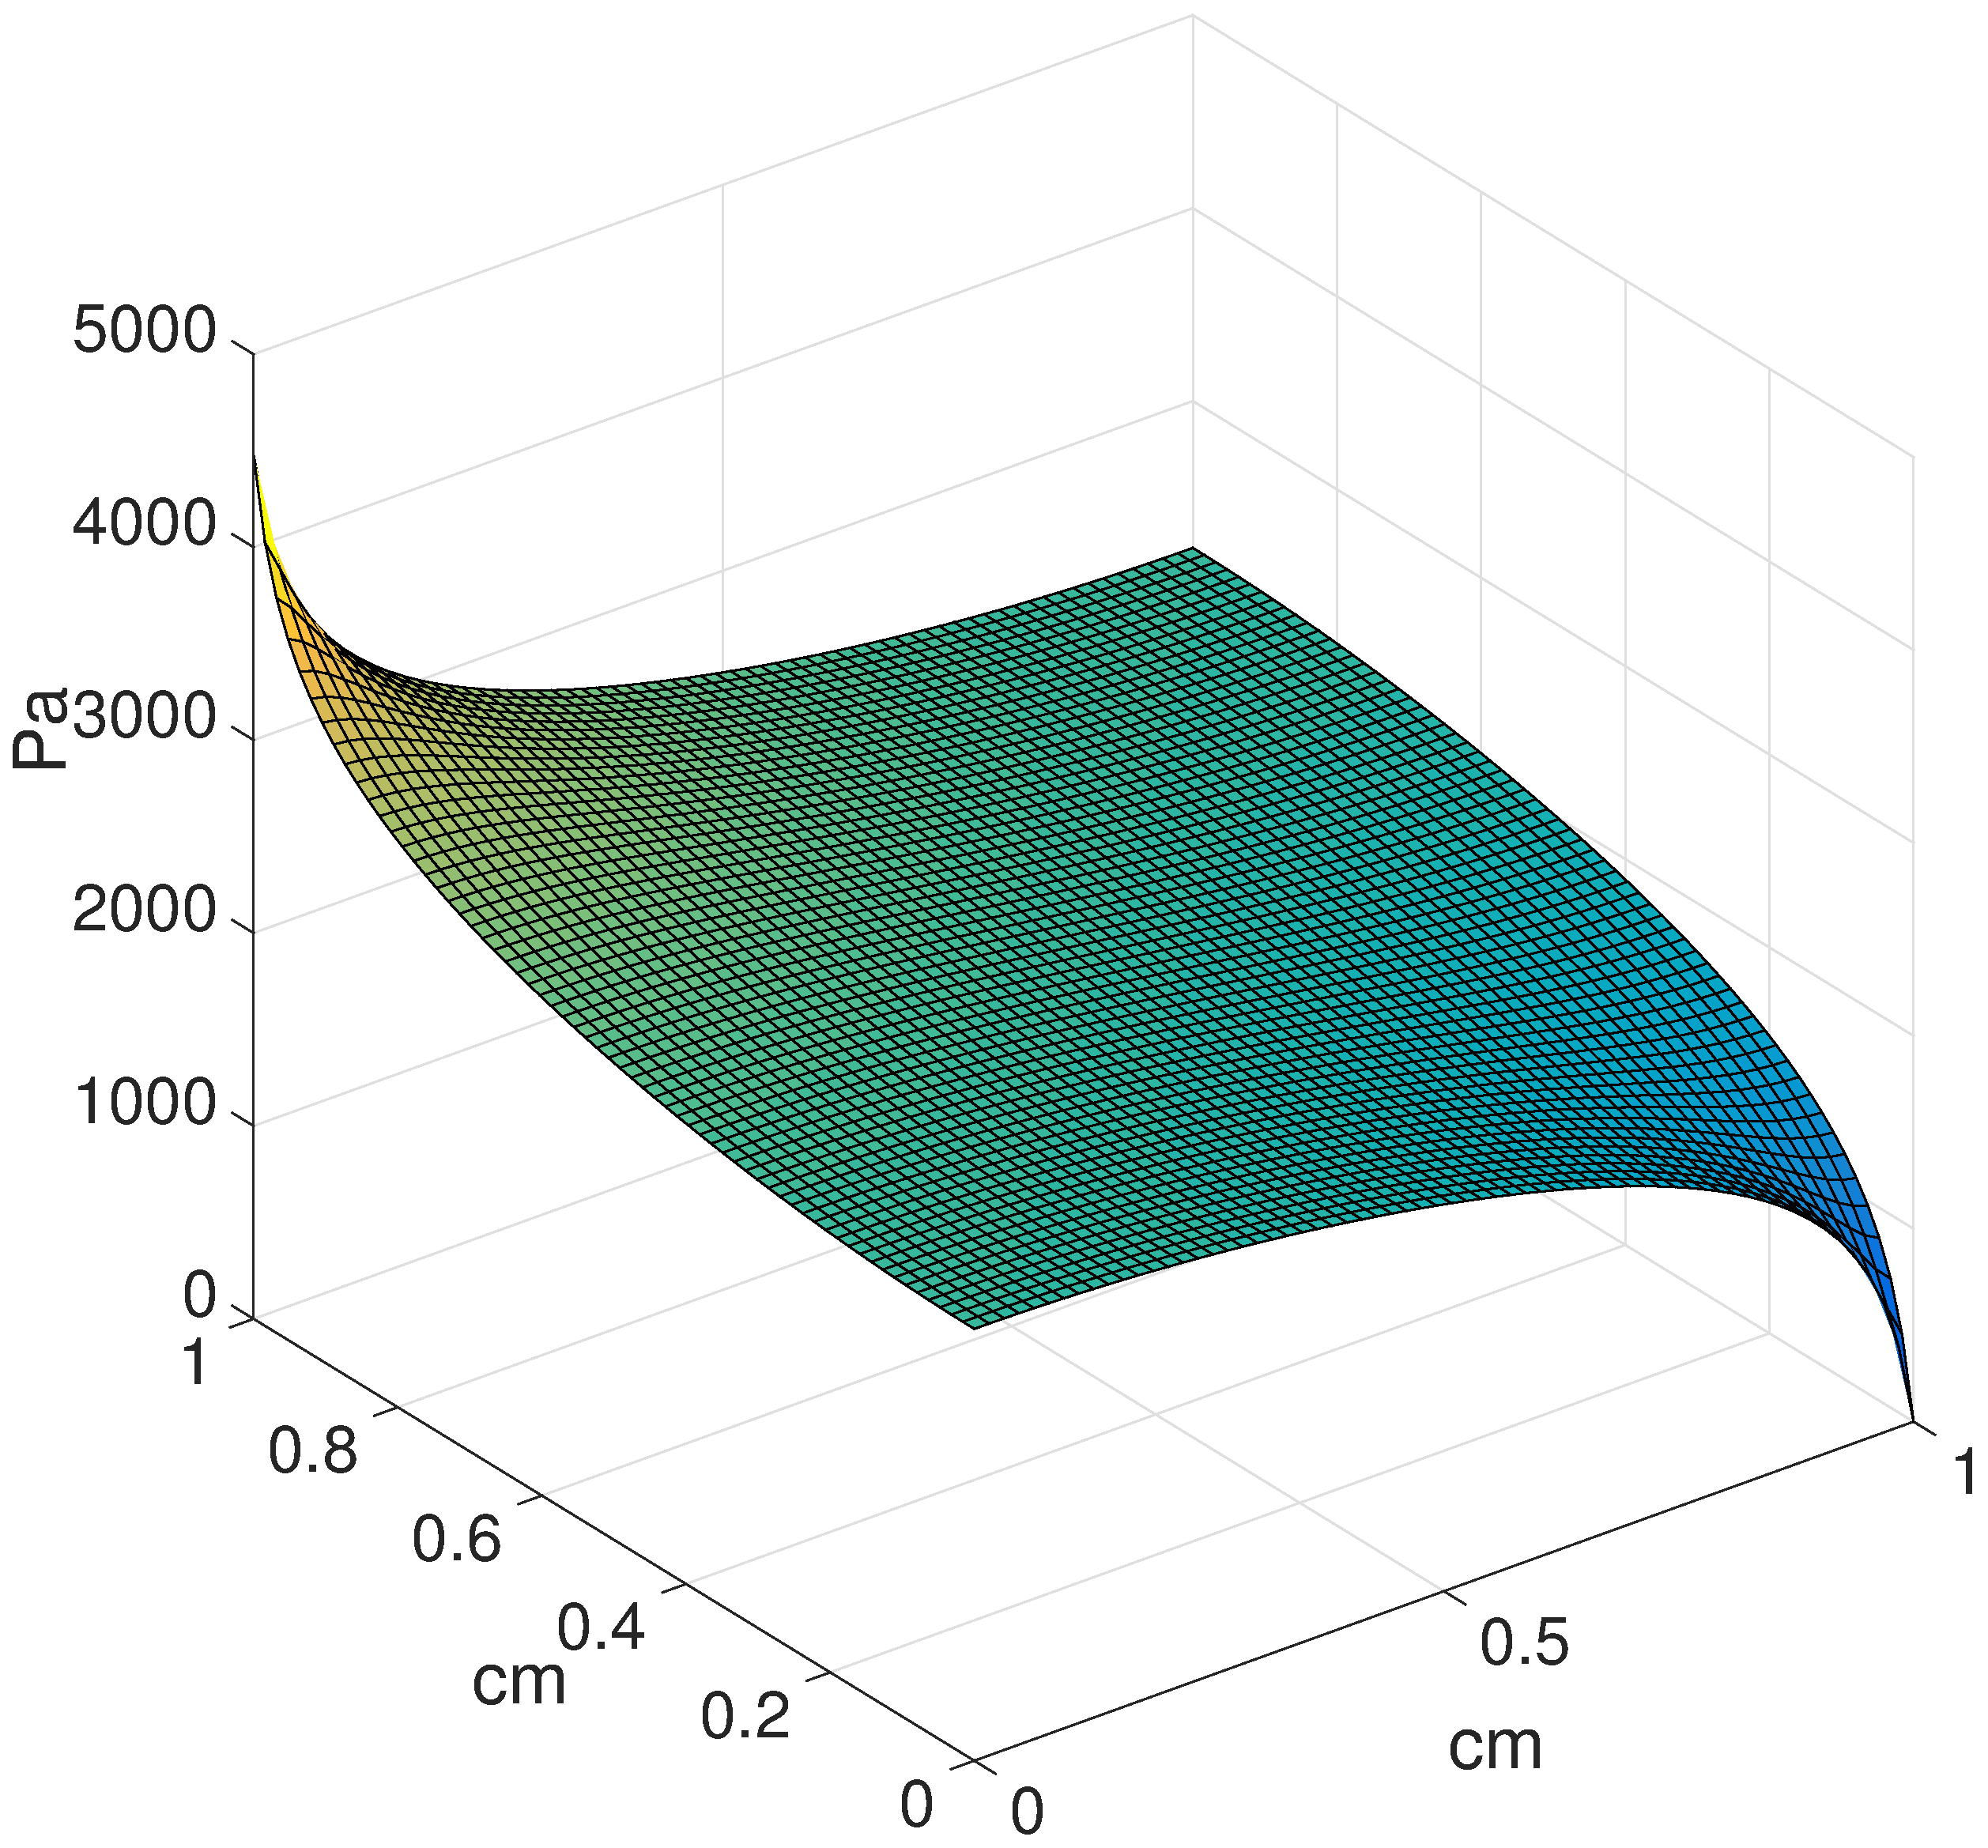
\includegraphics[width=.3\textwidth]{figs/pressure.eps} & 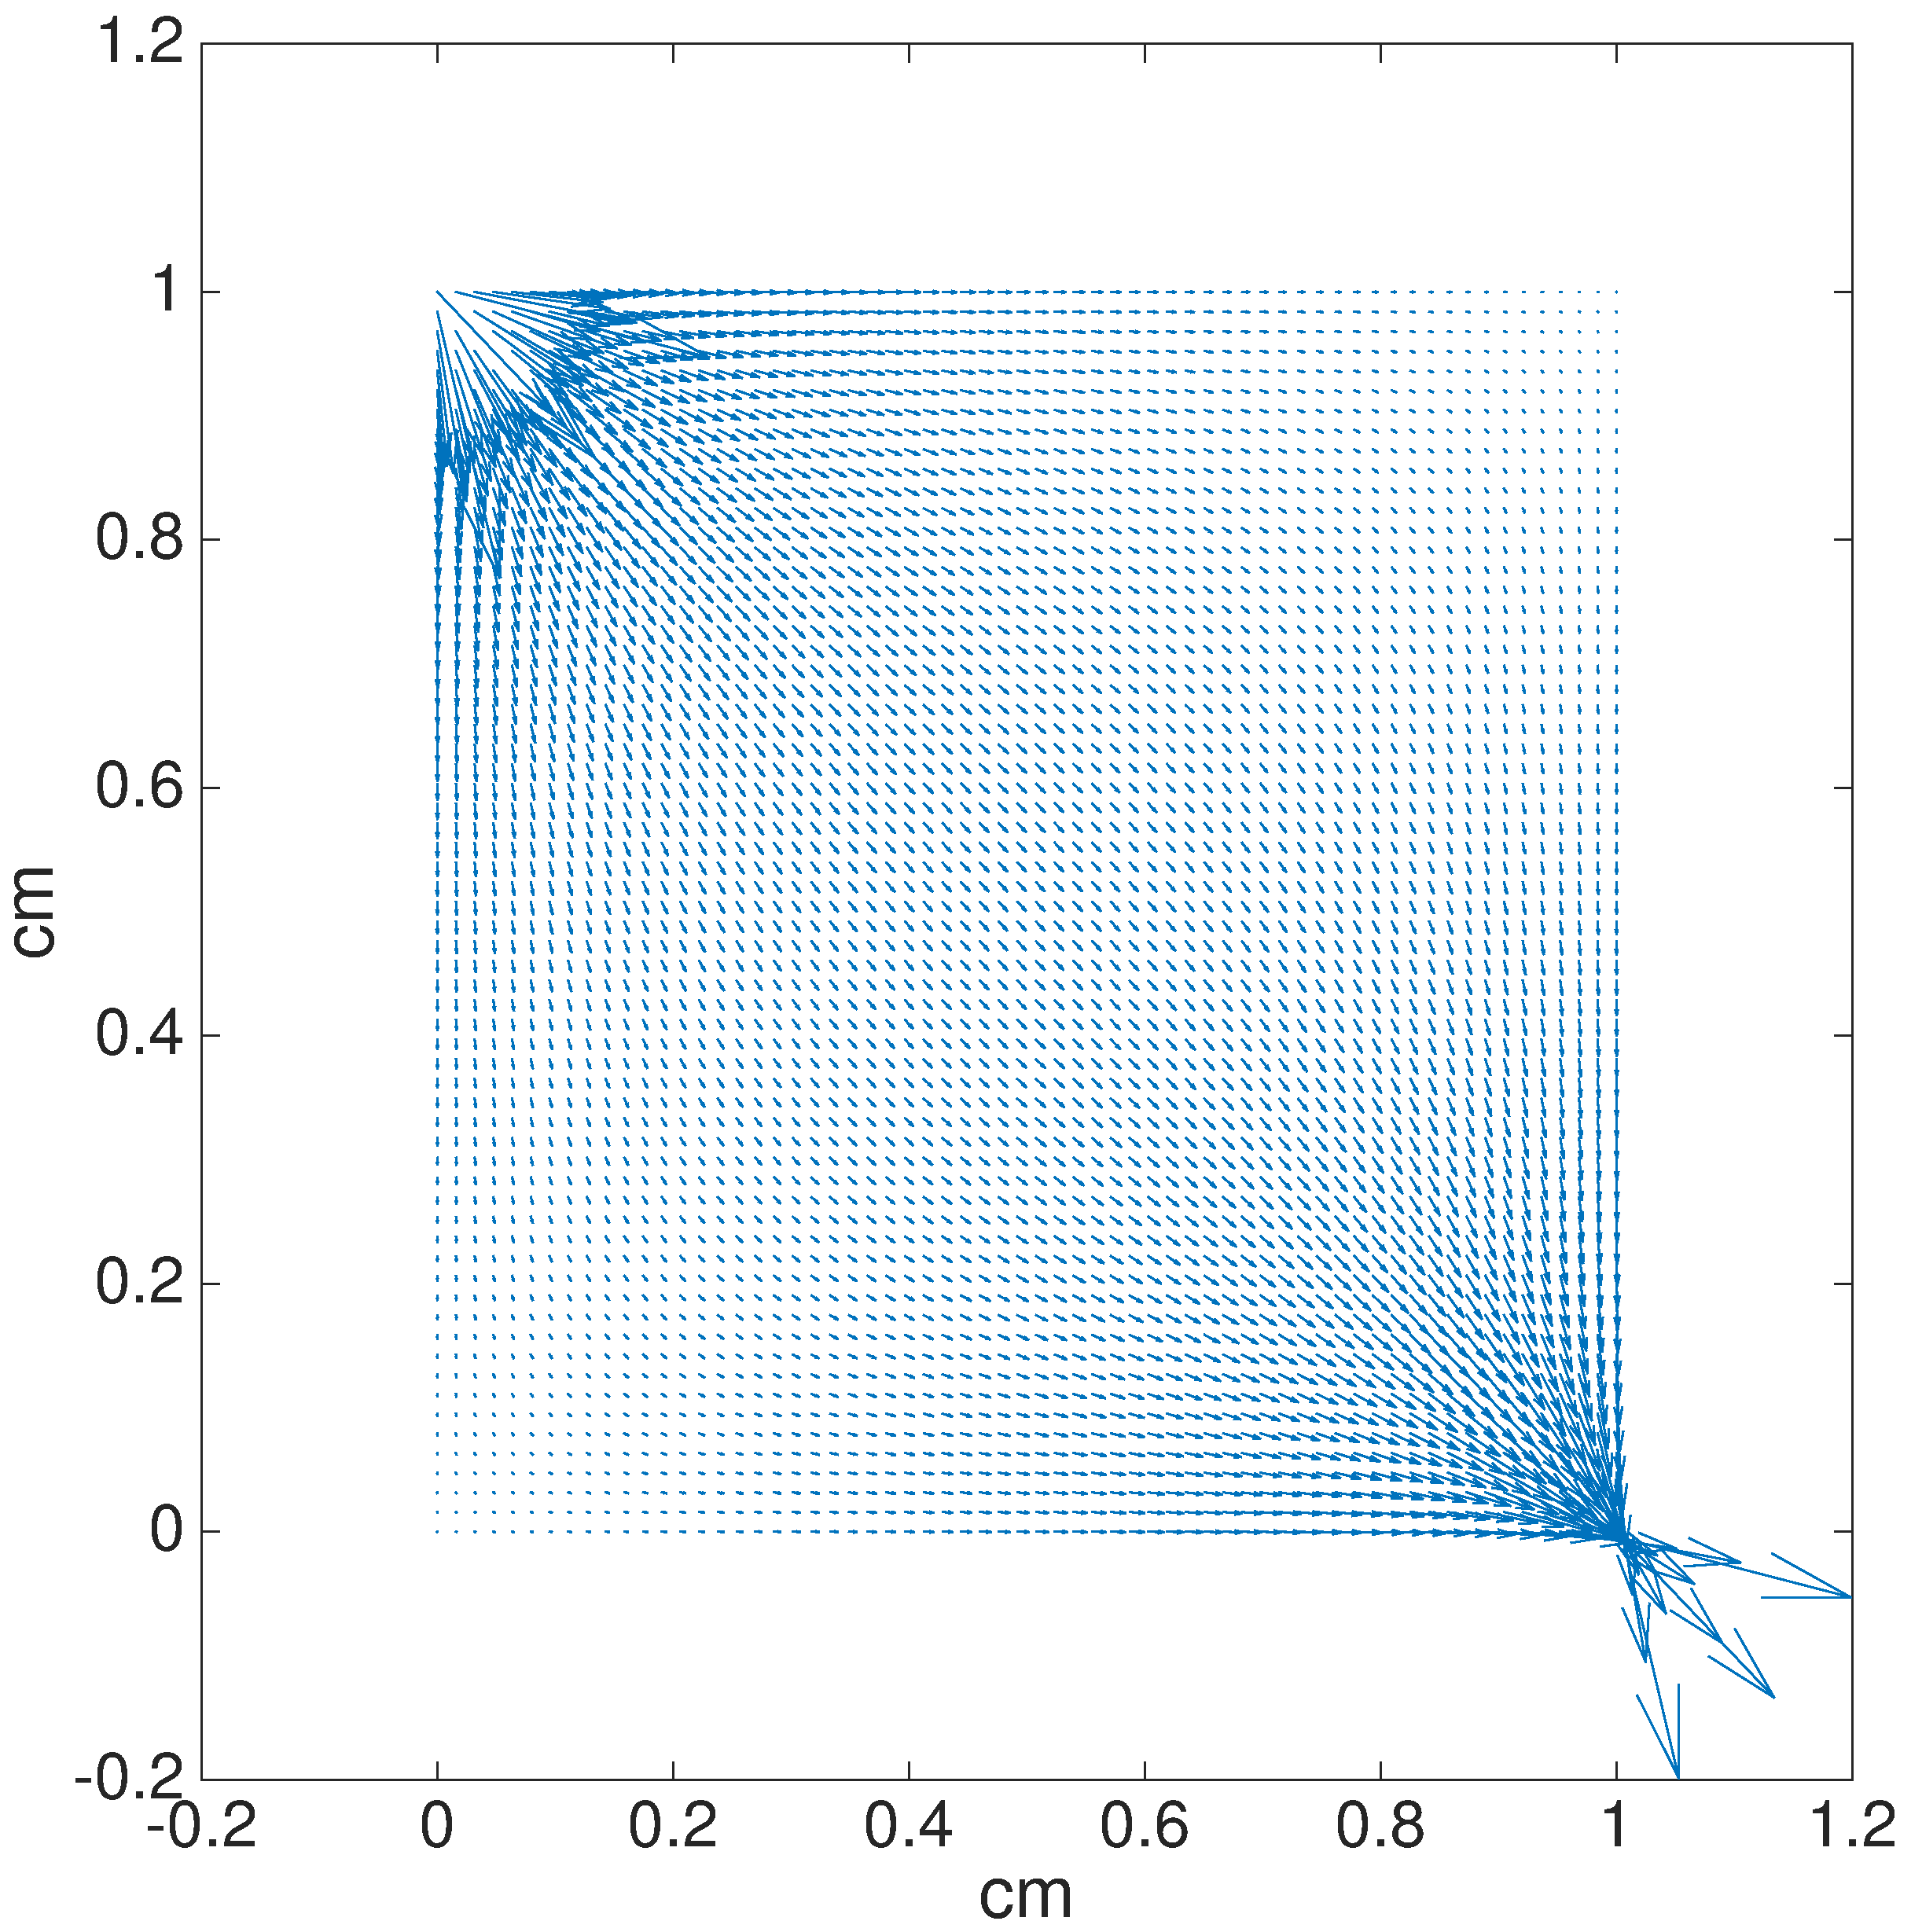
\includegraphics[width=.3\textwidth]{figs/flowQuiver.eps} & 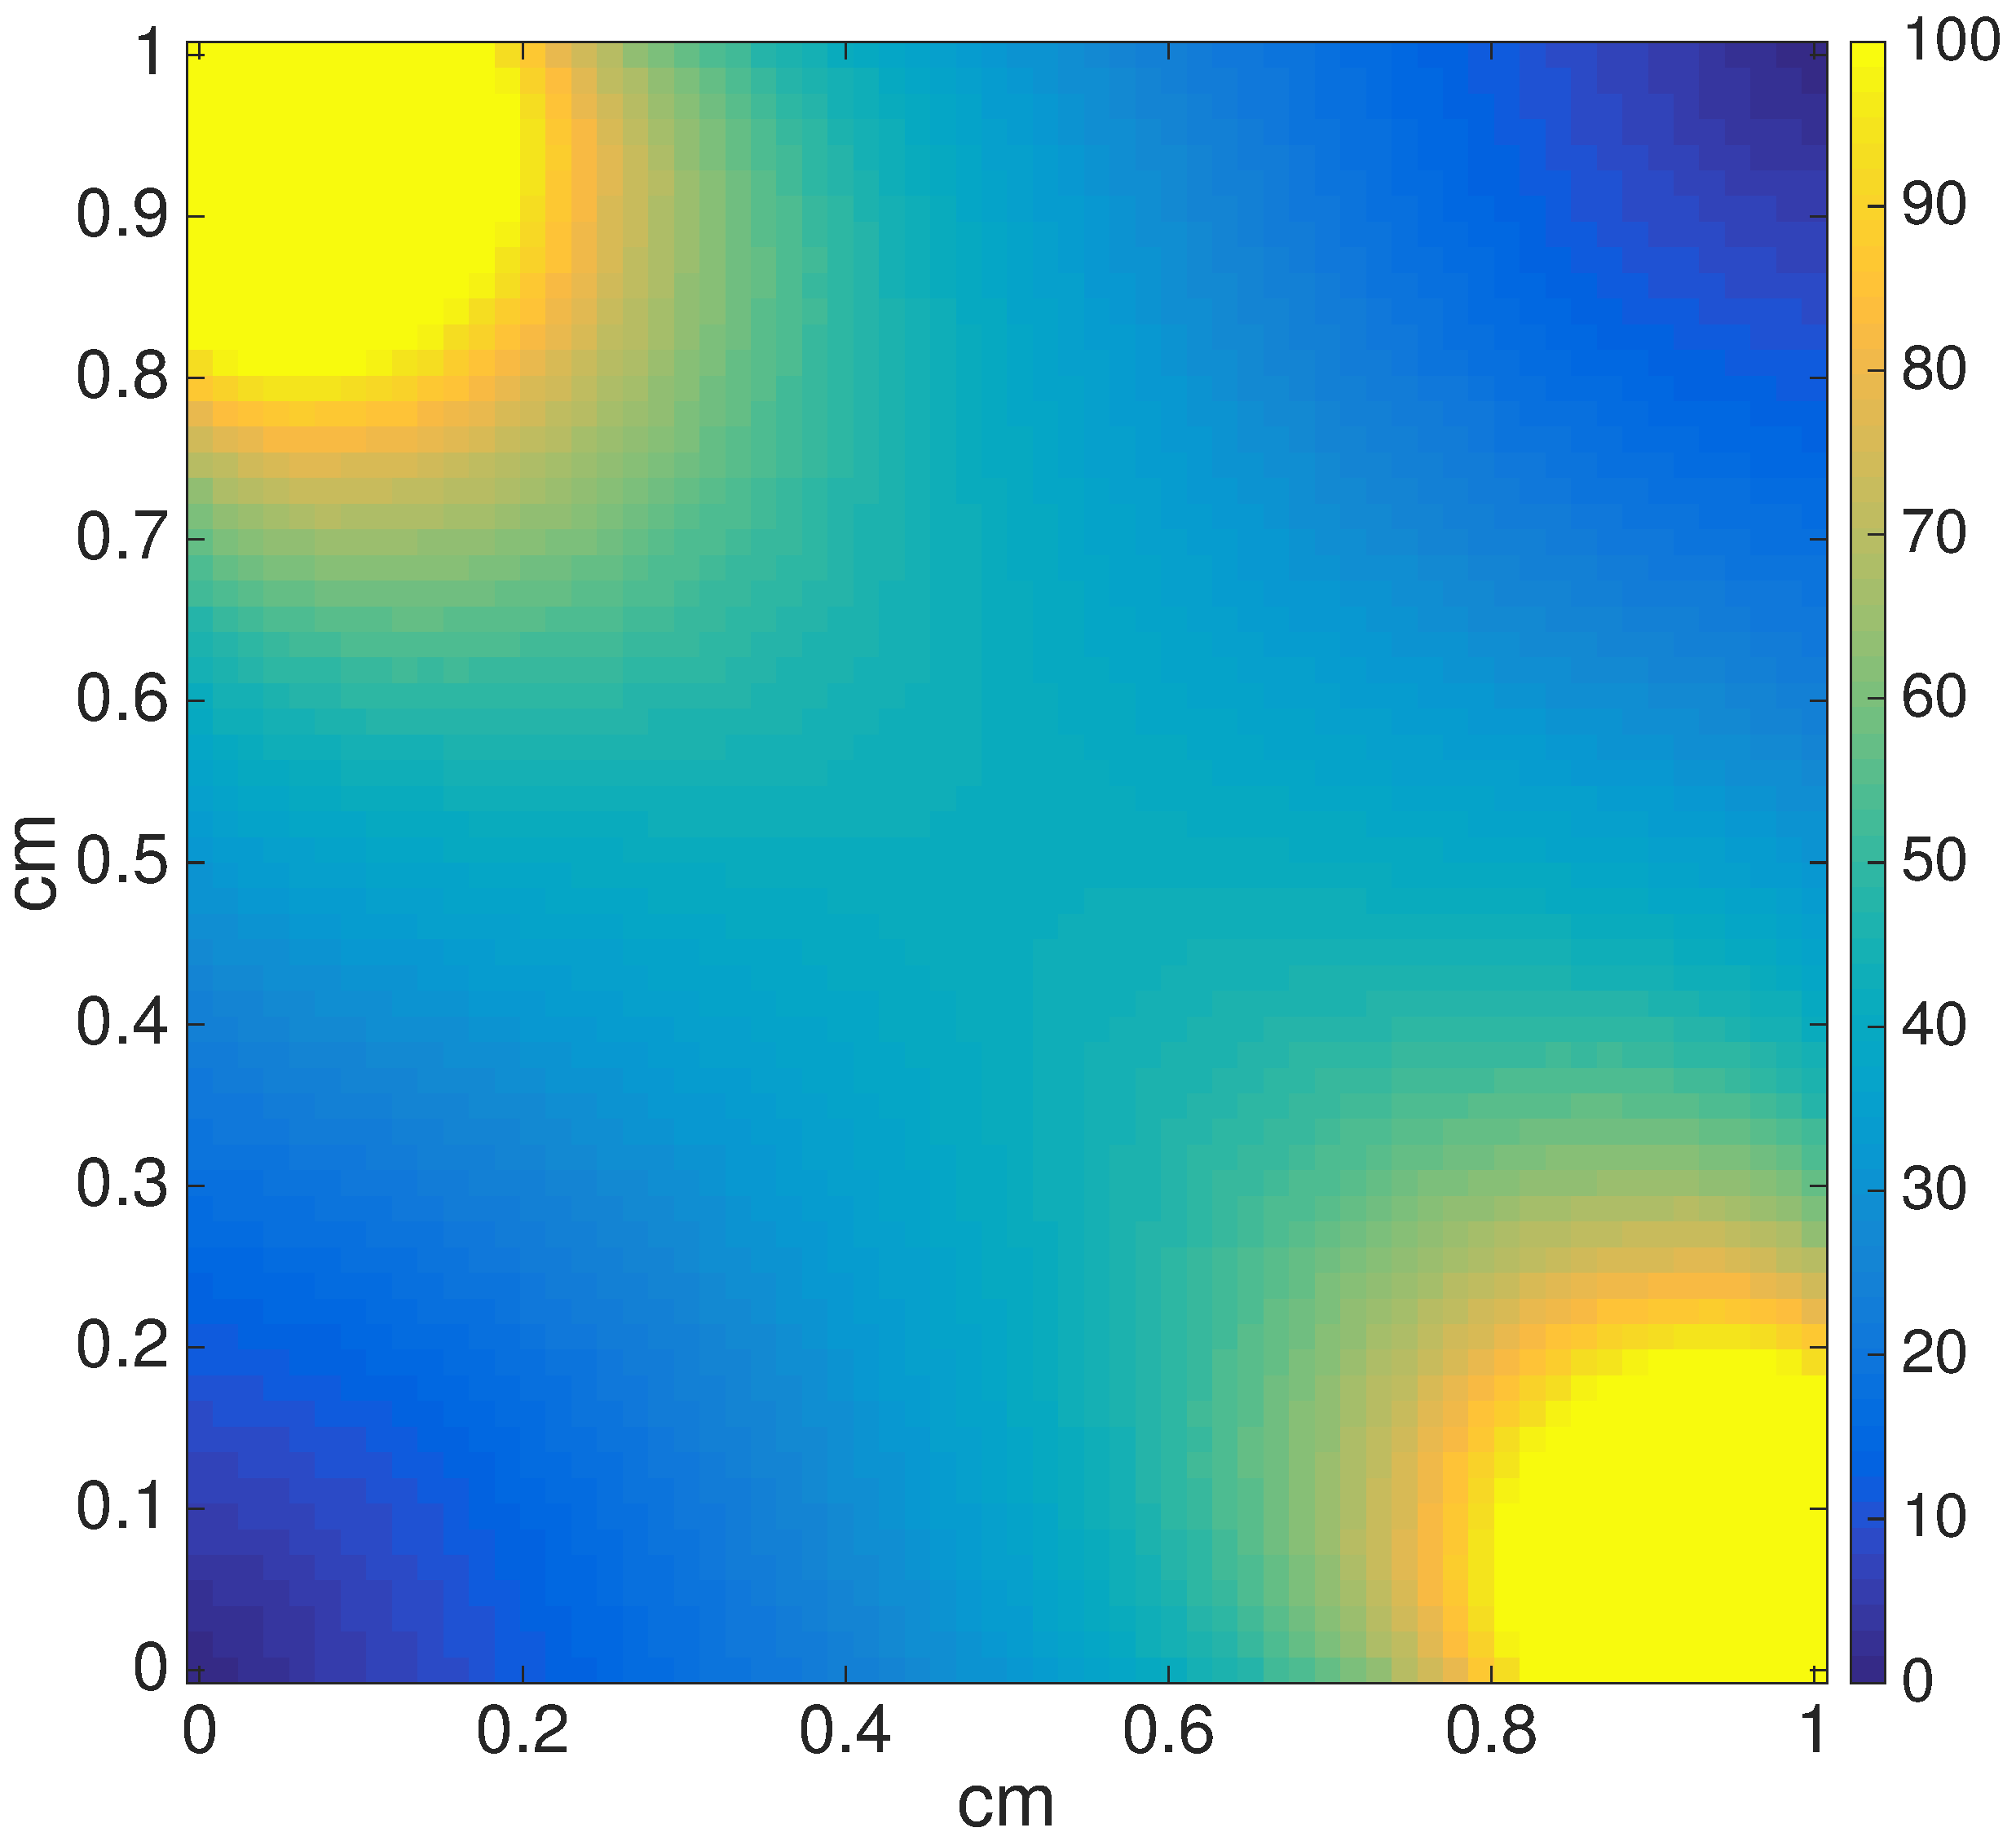
\includegraphics[width=.3\textwidth]{figs/perfusion.eps}\\
			(a) Pressure field $p$ & (b) Absolute flux & (c) Perfusion $P(x)$.
		\end{tabular}
    	\caption{Synthetic flow model with a source in the upper left corner and a sink in the lower right corner. (a) Pressure field [\si{\pascal}] from solving the linear system in \eqref{eq:flowmodel}  (b) vector valued absolute flux field $\int_{\partial \Omega_i}q ds$ [\si{\siq}], (c) Voxelwise perfusion $P(x)$ [\si{\siPml}] resulting from  the flux field, according to \eqref{eq:flux2perf}.}
	        \label{fig:flowpressureperfusion}
	\end{figure}
	
	\begin{figure}[H]
		\centering
		\begin{tabular}{c c}
			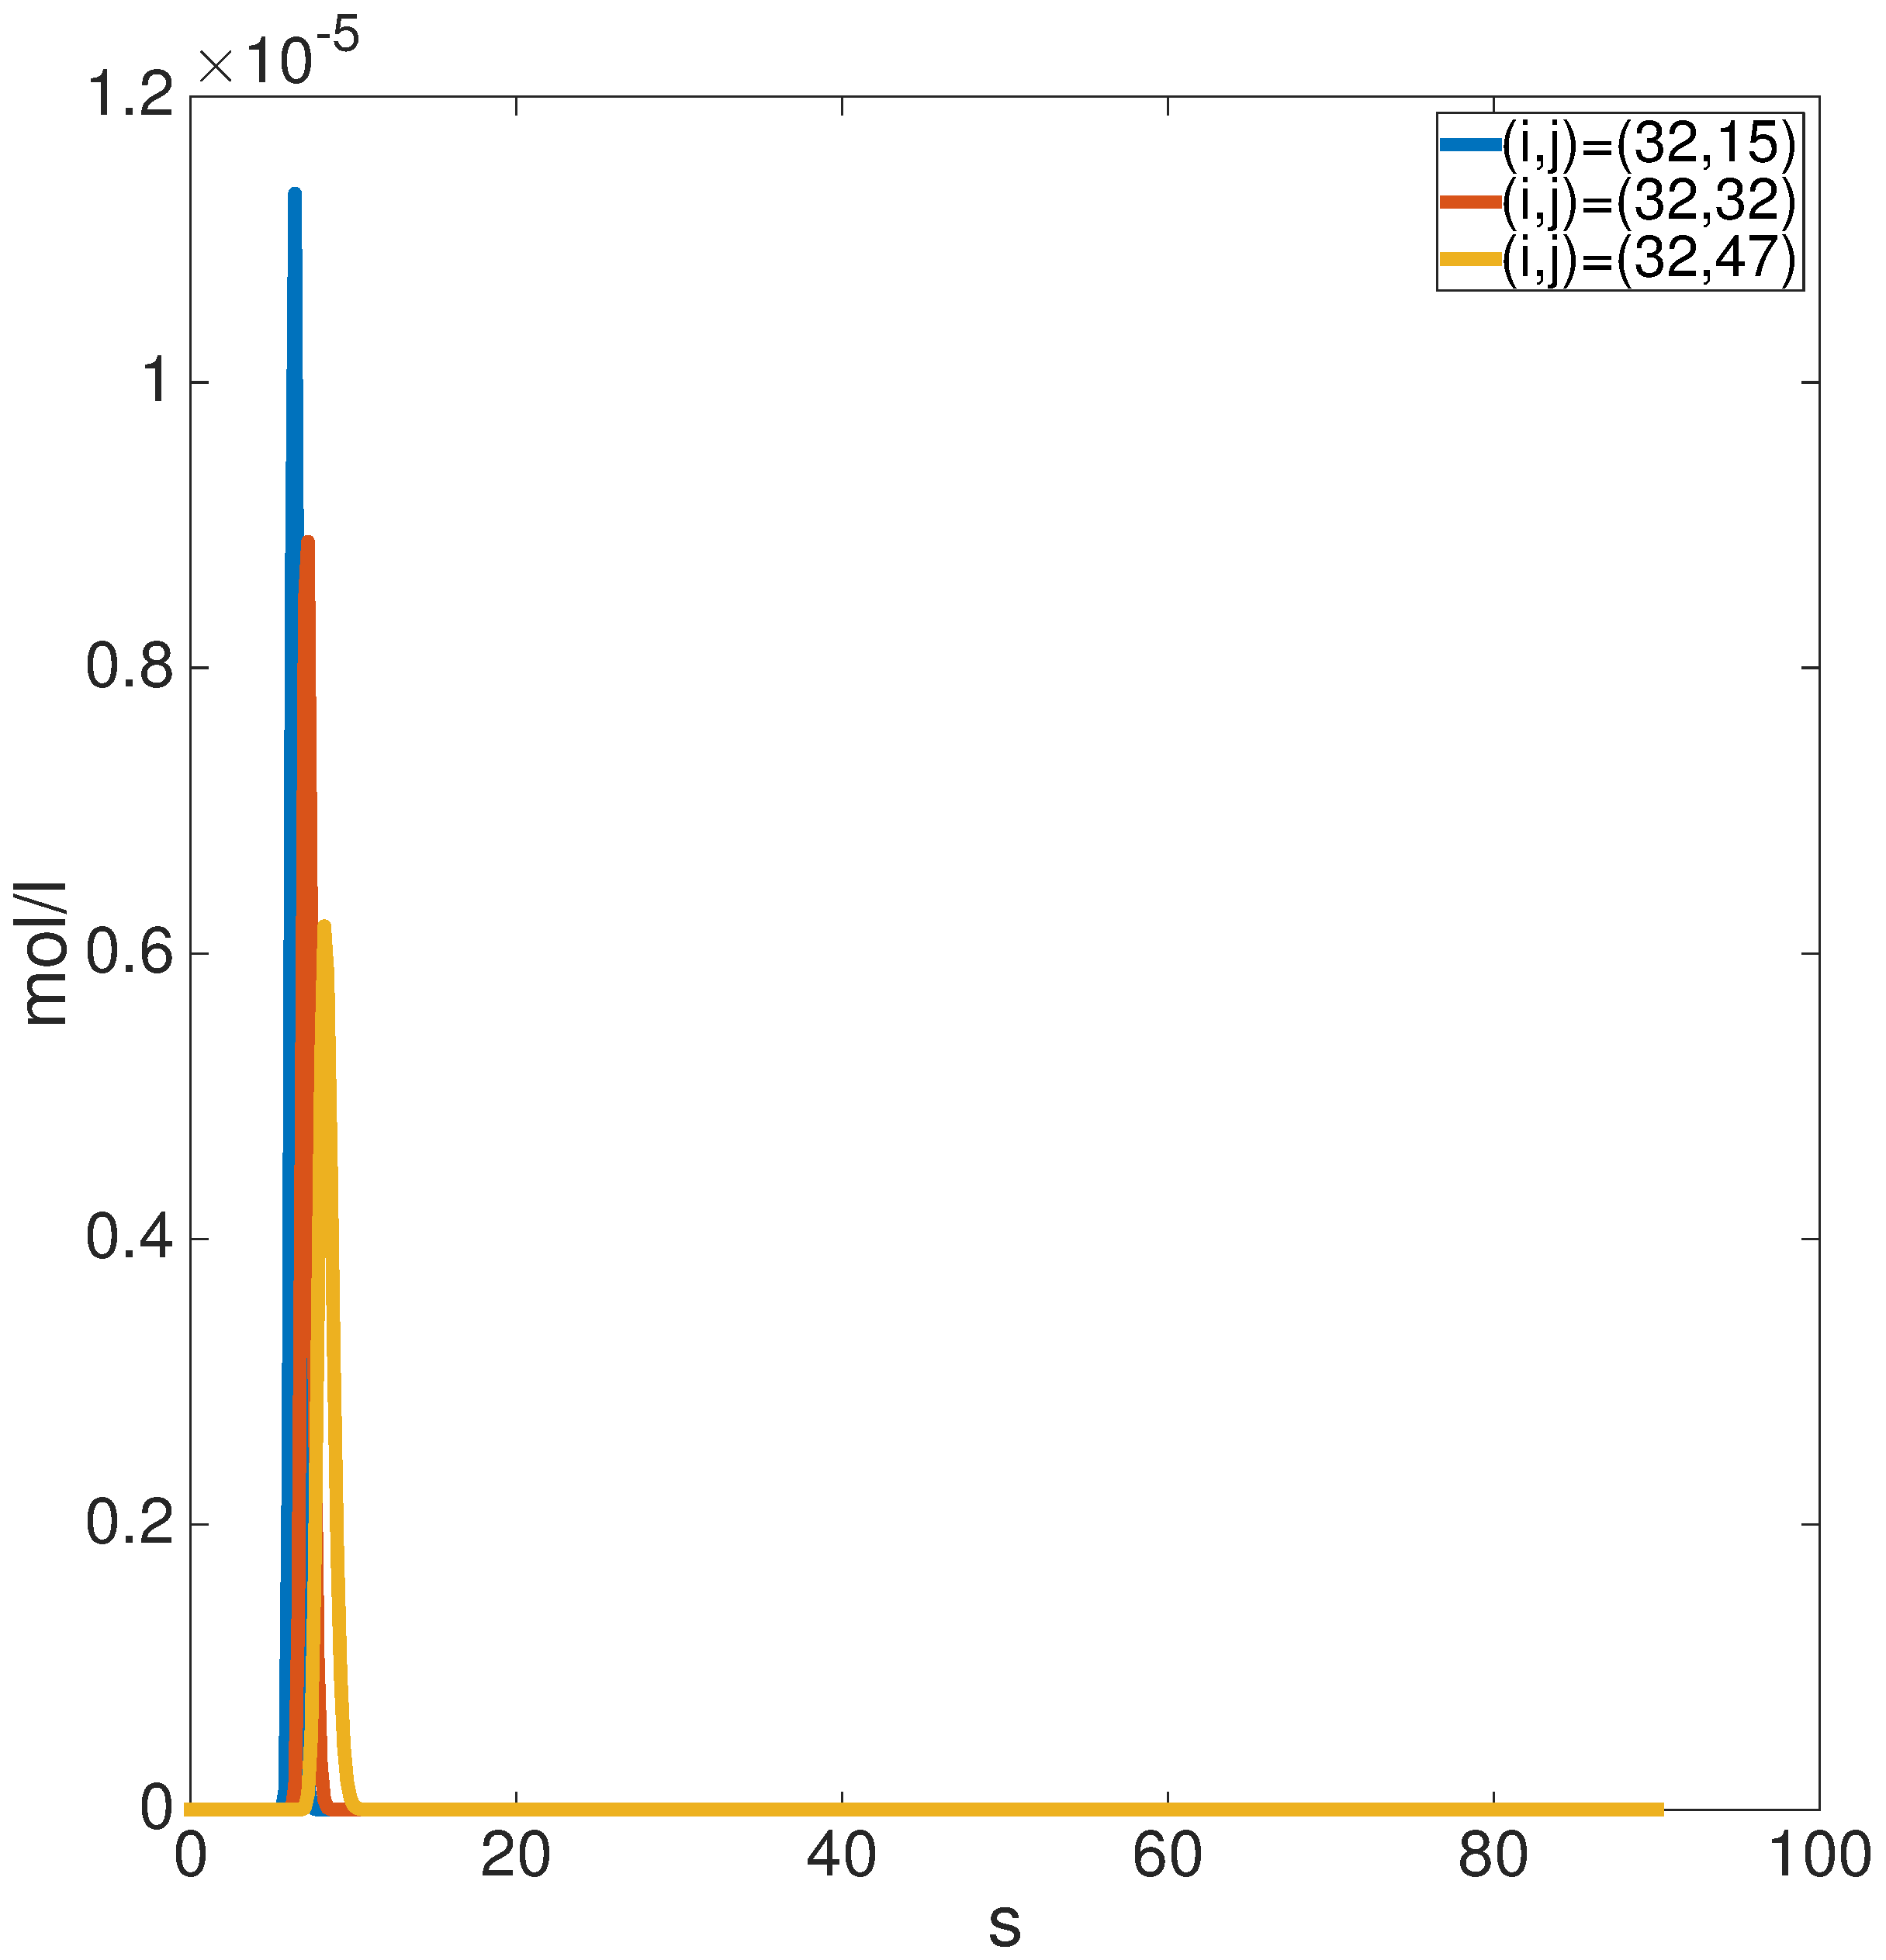
\includegraphics[width=.45\textwidth]{figs/PMM153247.eps} & 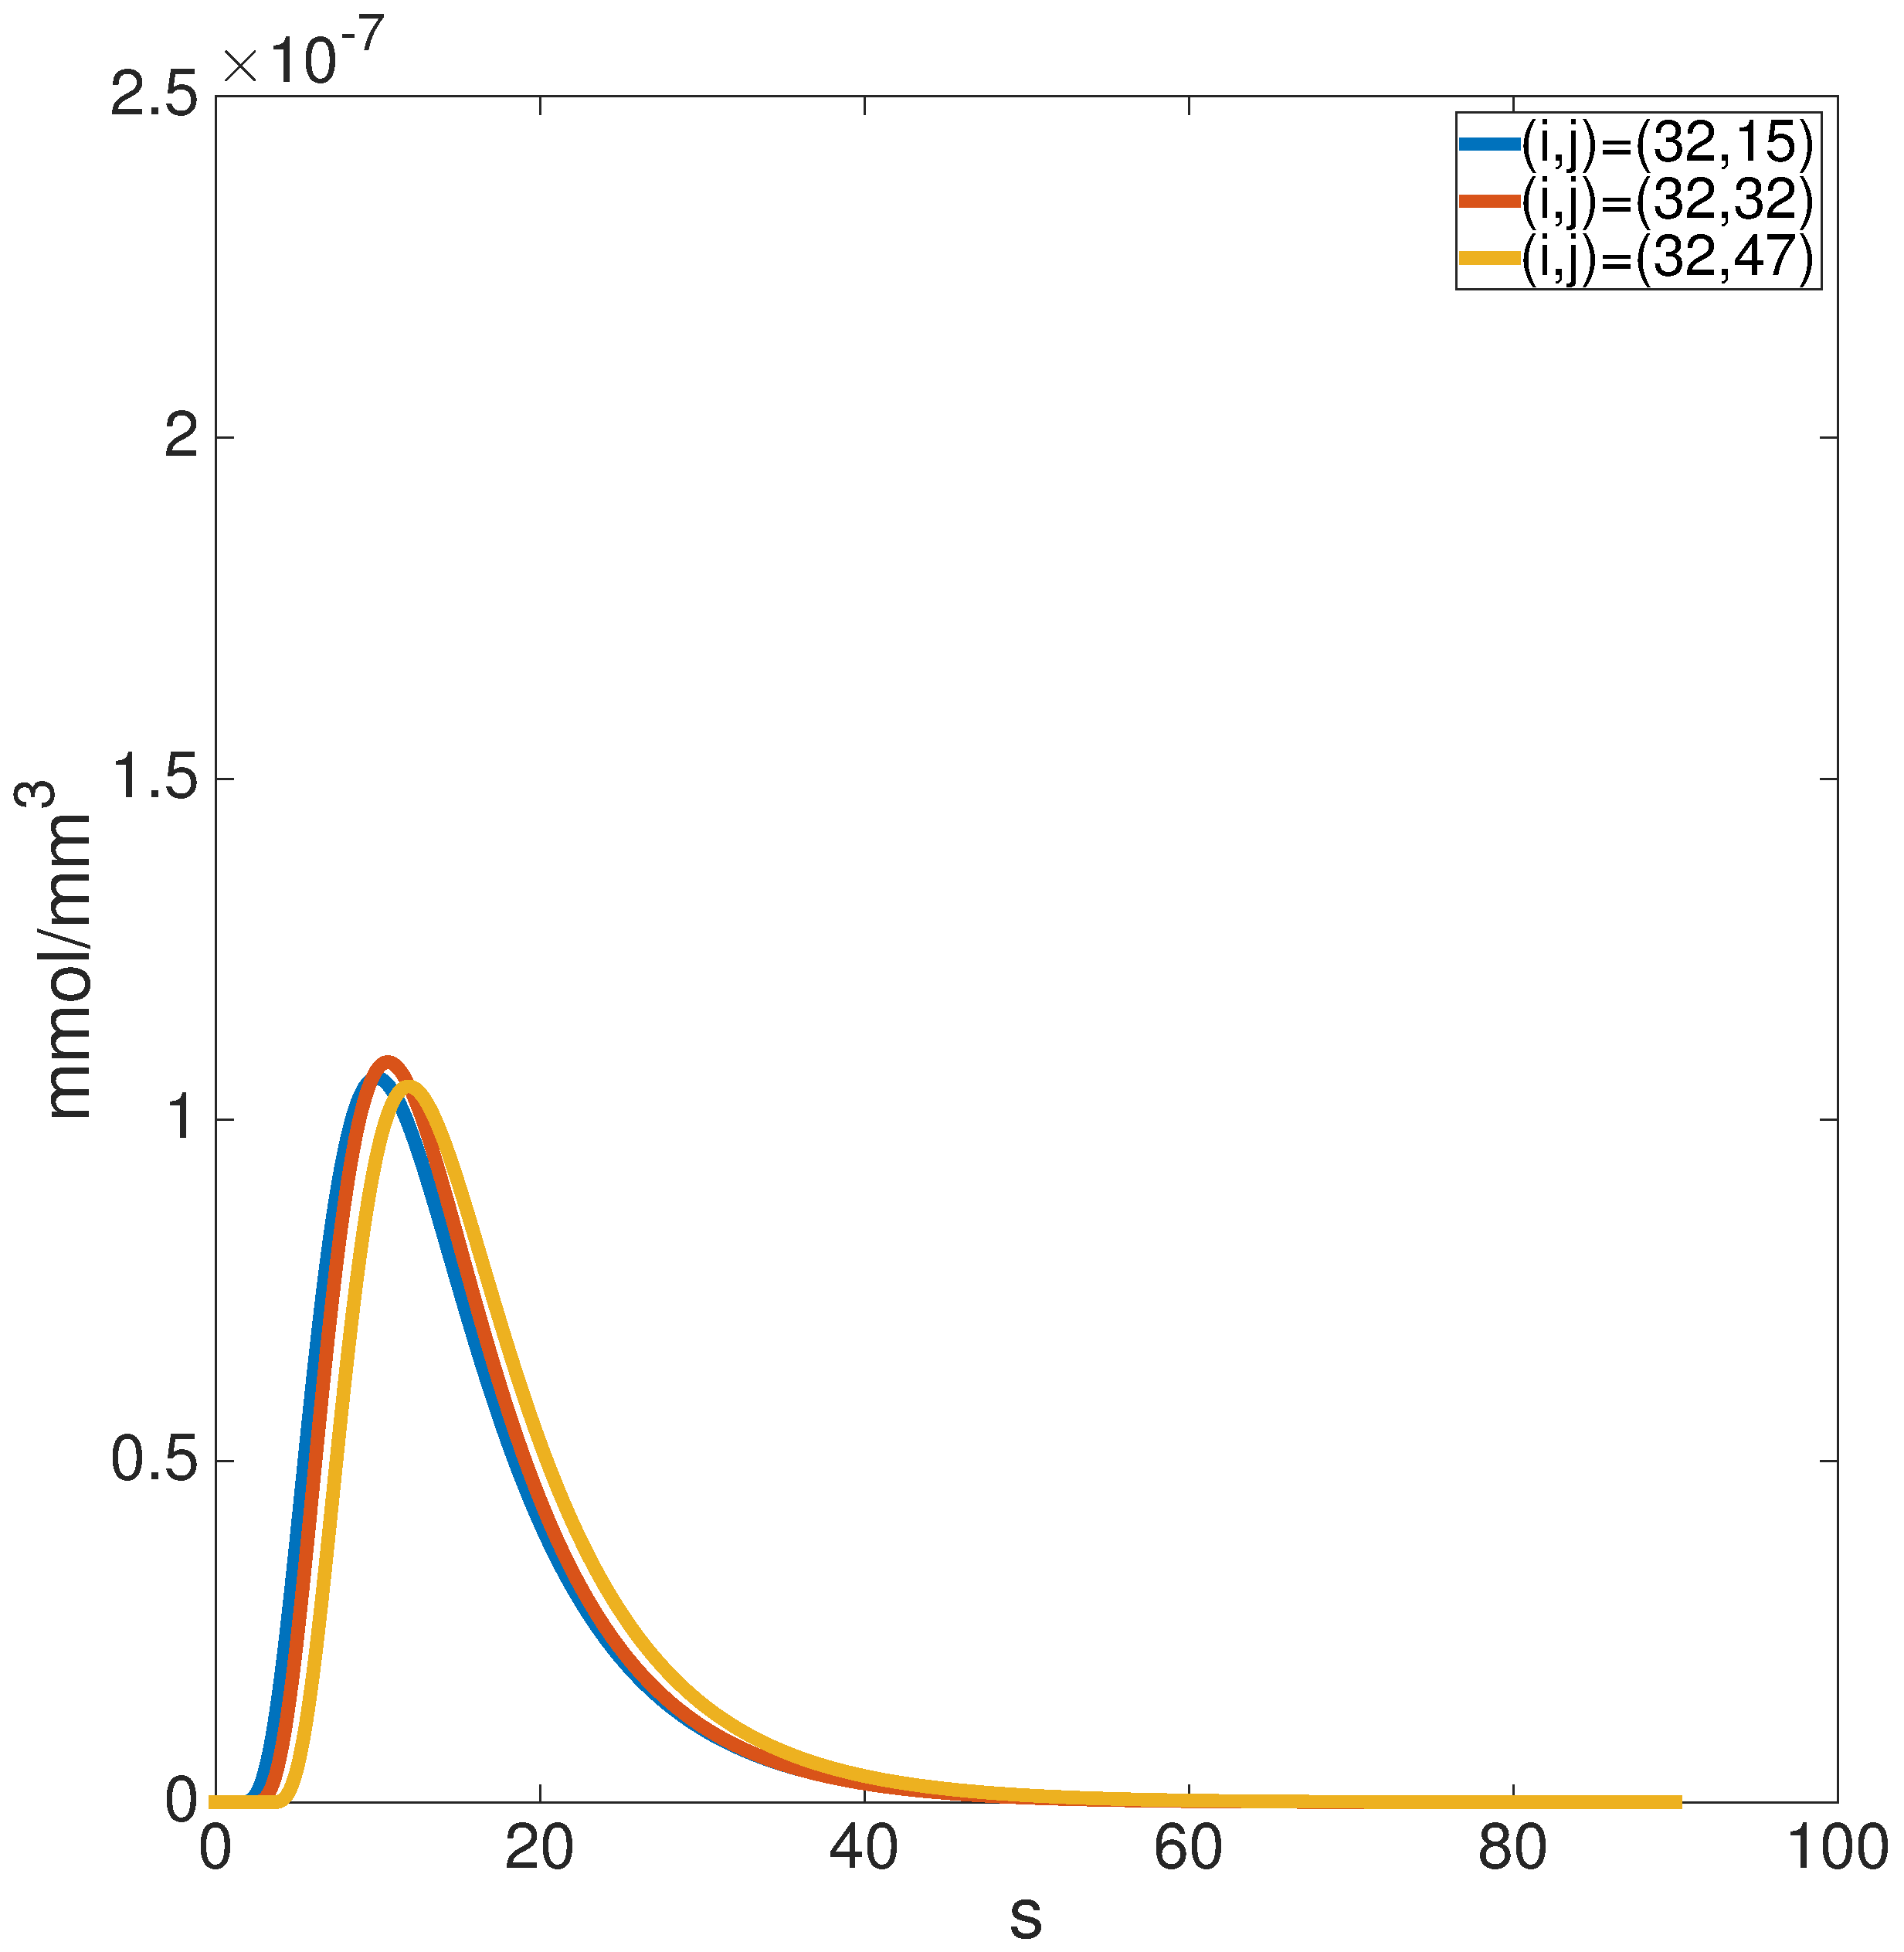
\includegraphics[width=.45\textwidth]{figs/convM153247.eps} \\
			(a) Porous Media Model & (b) Convolution Model
		\end{tabular}
		\caption{Comparison of tissue curves in the Porous Media (a) and the Convolution Model (b). Curves were sampled in the middle row $i=32$ and columns $j \in \{15,32,47\}$.}
		\label{fig:tissuecomp}
	\end{figure}
	
	

	%--------------------------------------------------
	%--------------------------------------------------
	% Section: Results
	%--------------------------------------------------
	%--------------------------------------------------
	\section{Results}\label{sec:results}

	We tested the the convolution based classical model \eqref{eq:conv} as well as maximum-slope model \eqref{eq:MS} for their capability to recover the perfusion values.
	The success of the restoration was measured voxelwise in terms of the relative error of the recovered perfusion with respect to the true perfusion
	\[
		RE := \frac{\vert P_{\mathrm{rec}} - P_{\mathrm{true}}\vert}{P_{\mathrm{true}}}\cdot 100\%.
	\]
	Prior to reconstruction, the input data was downsampled to a time-resolution of $\SI{.2}{\second}$.
	In order to simulate different spatial resolutions of the scanning process, the data was averaged using different block-sizes ranging from $(1,1)$ to $(64,64)$.
	Results are displayed in Figure \ref{fig:resultsPMM} as well as in Table \ref{tab:resultsSim}.
	Impuls response function reconstructed from the Porous Media Model are displayed in Figure \ref{fig:deconvResults}.	
	
	\begin{table}[H]
		\caption{Results of the perfusion restoration with median relative errors in percent. Relative error was computed block-wise as $\vert P_{\mathrm{rec}} - P_{\mathrm{true}}\vert / P_{\mathrm{true}}\cdot 100\%$. Displayed is the median RE over the entire domain. Abbreviations are: PMM - Porous Media Model, ConvM - Convolution Model.}
		\centering
		\begin{tabular}{l c c c c c }
			& Model & \multicolumn{4}{c}{Block Size}\\
			 					 			& 		& (1,1) 	& (5,5)		& (10,10)	& entire domain \\
			\toprule
			\multirow{2}{*}{PMM: Perfusion} & MS 	& $170.09$ 	& $165.03$ 	& $158.57$	& $2.65$ \\
			 					 	   		& bSVD  & $859.06$ 	& $768.58$ 	& $664.84$	& $1.25$ \\
			\multirow{2}{*}{ConvM: Perfusion} & MS 	& $23.20$ 	& $24.26$ 	& $25.75$ 	& $37.96$ \\
			 					 			& bSVD  & $2.43$ 	& $4.27$ 	& $8.80$ 	& $20.72$ \\
			\midrule											
			PMM: CBV & & $4.37\cdot10^{-5}$      & $4.37\cdot10^{-5}$		& $4.37\cdot10^{-5}$		& $4.37\cdot10^{-5}$ \\											
			ConvM:  CBV & & $1.94\cdot10^{-2}$   & $1.93\cdot10^{-2}$		& $2.12\cdot10^{-2}$		& $1.13$ 			
		\end{tabular}
		\label{tab:resultsSim}
	\end{table}


	\newcommand{\rbox}[2]{\rotatebox{90}{\hspace{#1}\mbox{\large #2}}}
	\begin{figure}[H]
		\centering
		\begin{tabular}{c c c c}
			 \rbox{0ex}{True perfusion} & 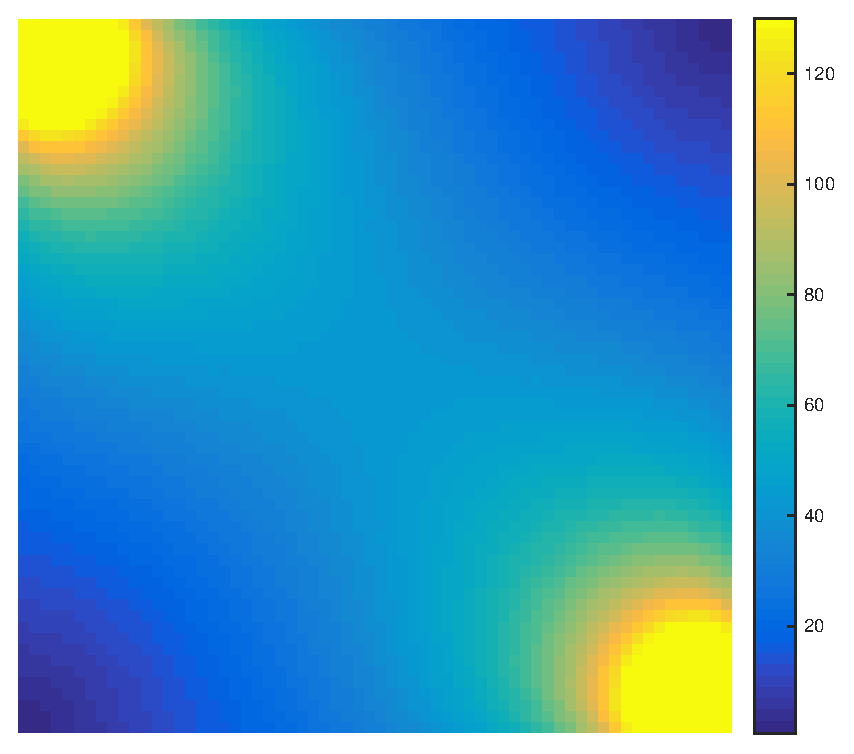
\includegraphics[width = .25\textwidth]{./figs/recTrue-PDE-1.eps} & 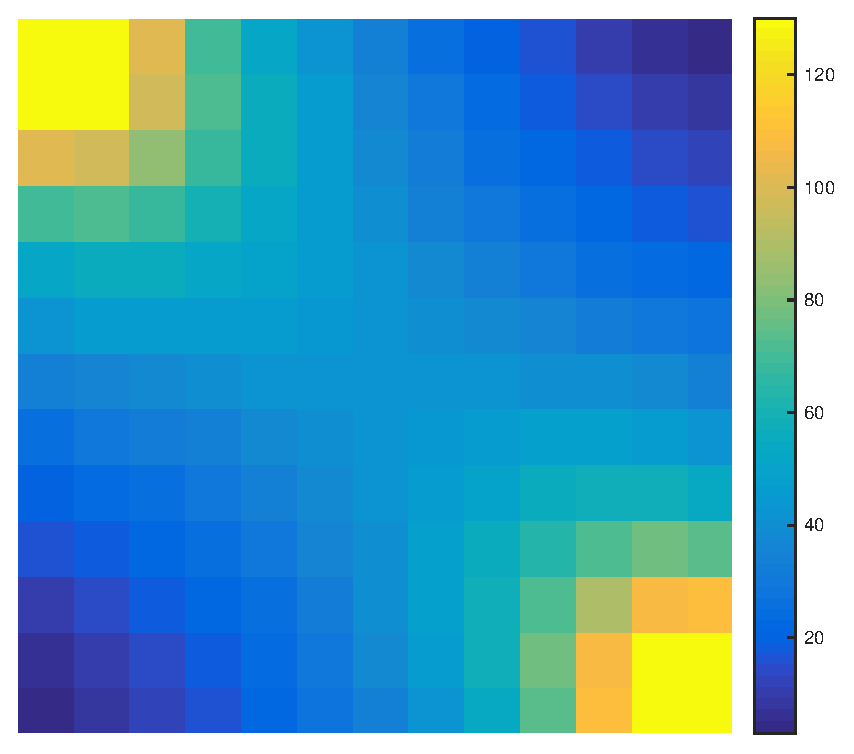
\includegraphics[width = .25\textwidth]{./figs/recTrue-PDE-5.eps} & 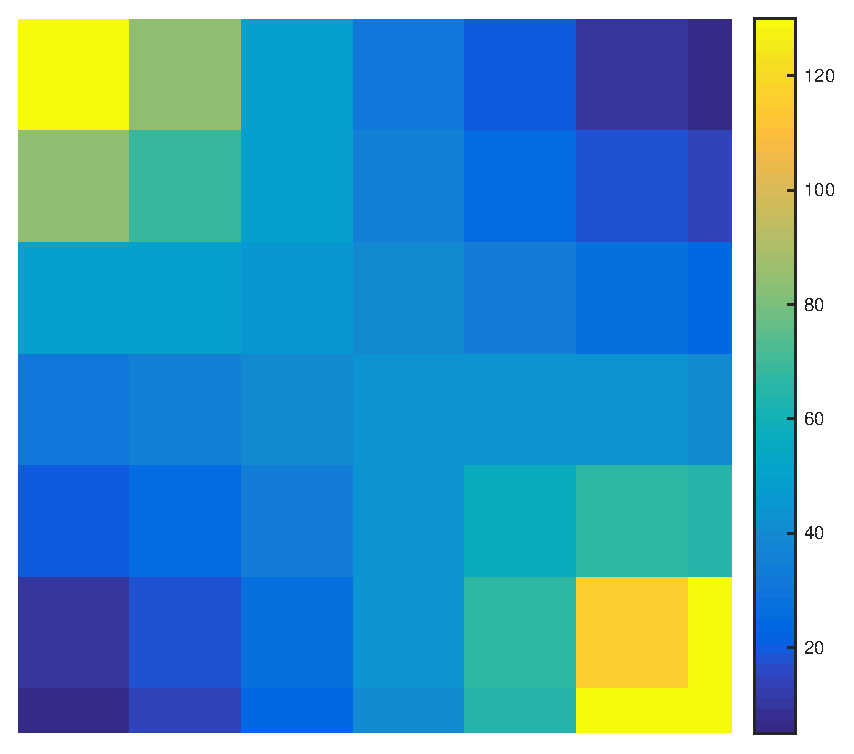
\includegraphics[width = .25\textwidth]{./figs/recTrue-PDE-10.eps}\\
			 \rbox{5ex}{bSVD} & 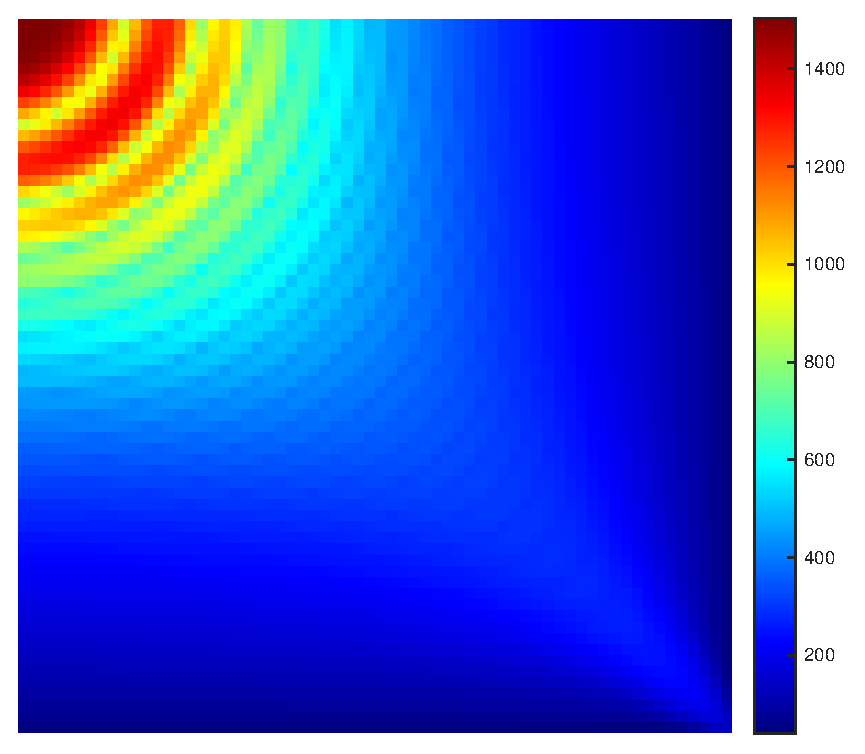
\includegraphics[width = .25\textwidth]{./figs/recCirc-PDE-1.eps} & 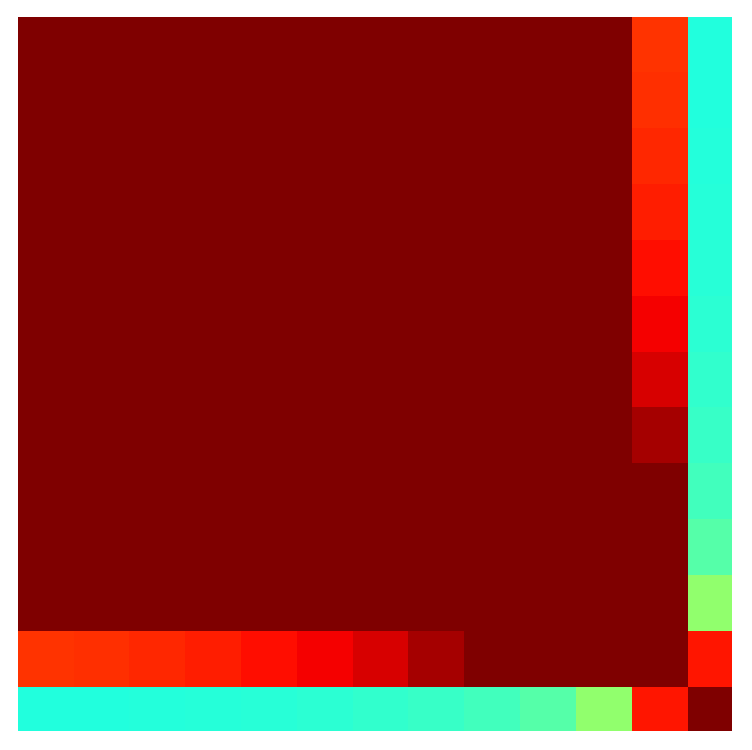
\includegraphics[width = .25\textwidth]{./figs/recCirc-PDE-5.eps} & 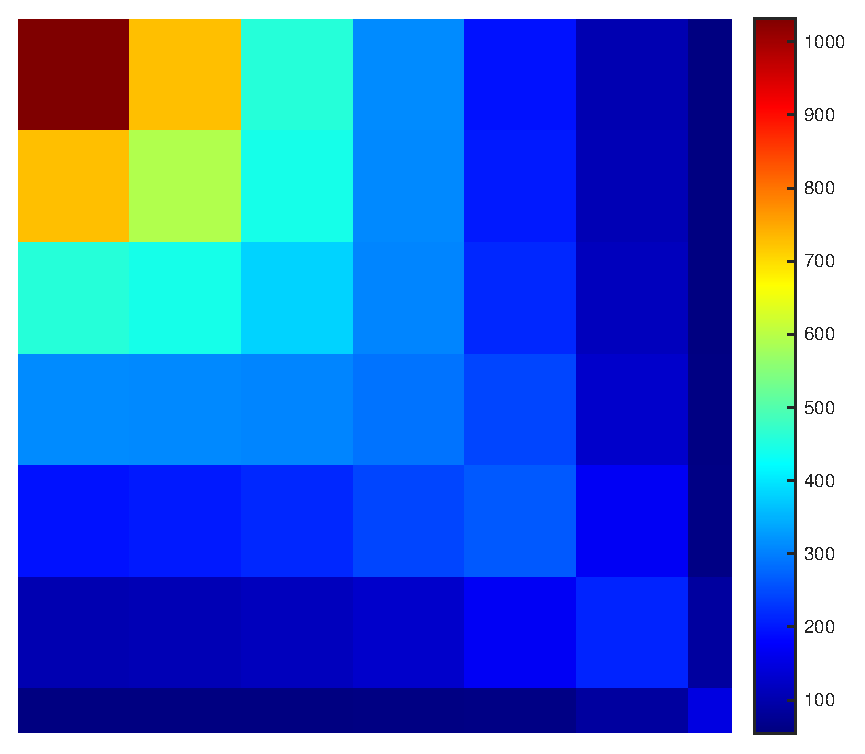
\includegraphics[width = .25\textwidth]{./figs/recCirc-PDE-10.eps}\\
			 \rbox{8ex}{MS} & 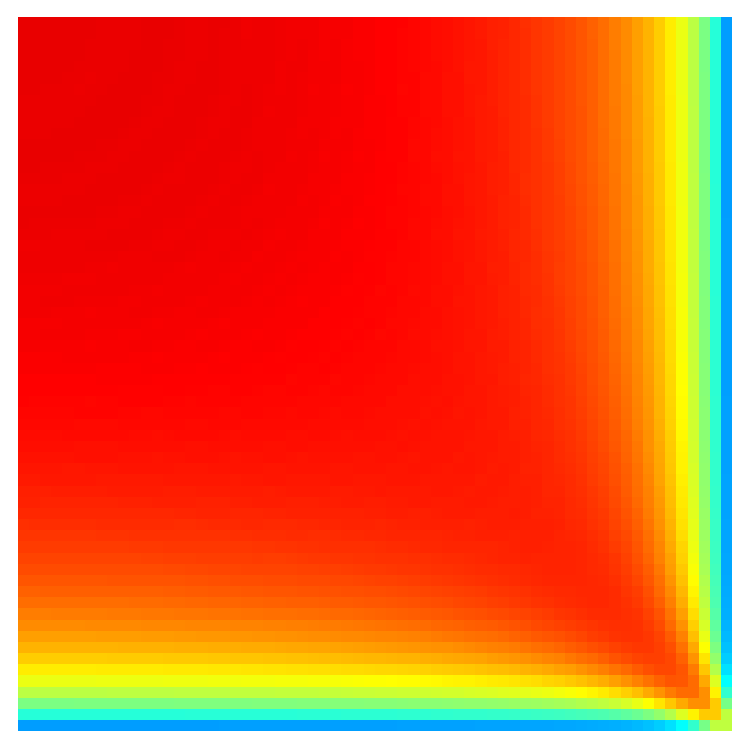
\includegraphics[width = .25\textwidth]{./figs/recMS-PDE-1.eps} & 
\includegraphics[width = .25\textwidth]{./figs/recMS-PDE-5.eps} & 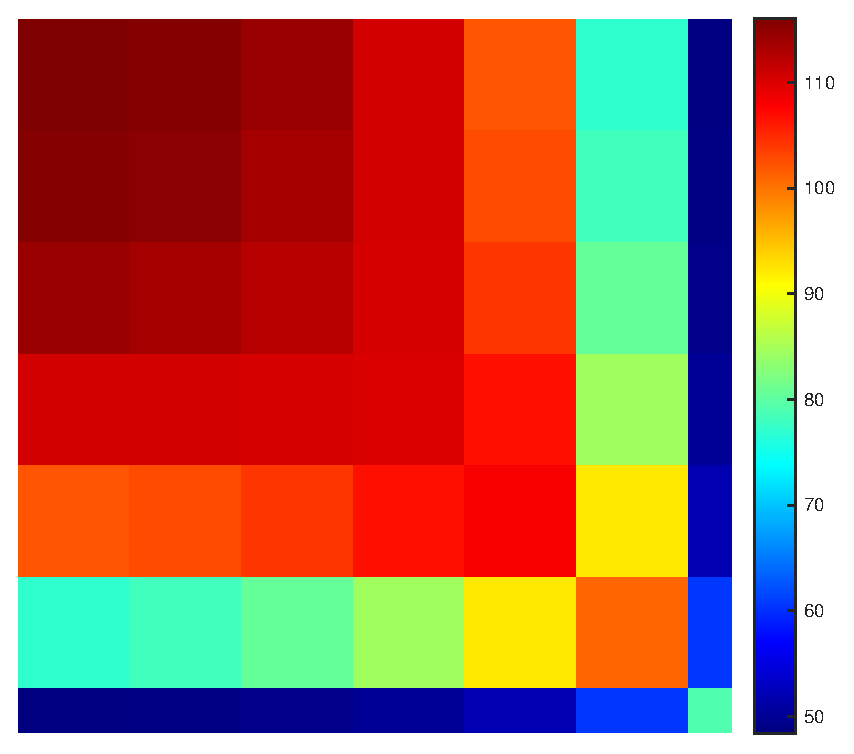
\includegraphics[width = .25\textwidth]{./figs/recMS-PDE-10.eps}\\			 			 			  
			   & (1,1) & (5,5) & (10,10)
		\end{tabular}
		\caption{Results of the restoration of perfusion for the Porous Media Model (PMM) for different levels of discretization, displayed in the columns. All results are given in $\mathrm{ml/min/100ml}$. First Row: Ground-Truth Perfusion (cf. Section \ref{sec:flux2perf}). Second Row: Perfusion as estimated by bSVD. Third Row: Perfusion as estimated by the Maximum-Slope model.}	
		\label{fig:resultsPMM}			
	\end{figure}



	\begin{figure}[H]
		\centering
			\begin{tabular}{c c}
				 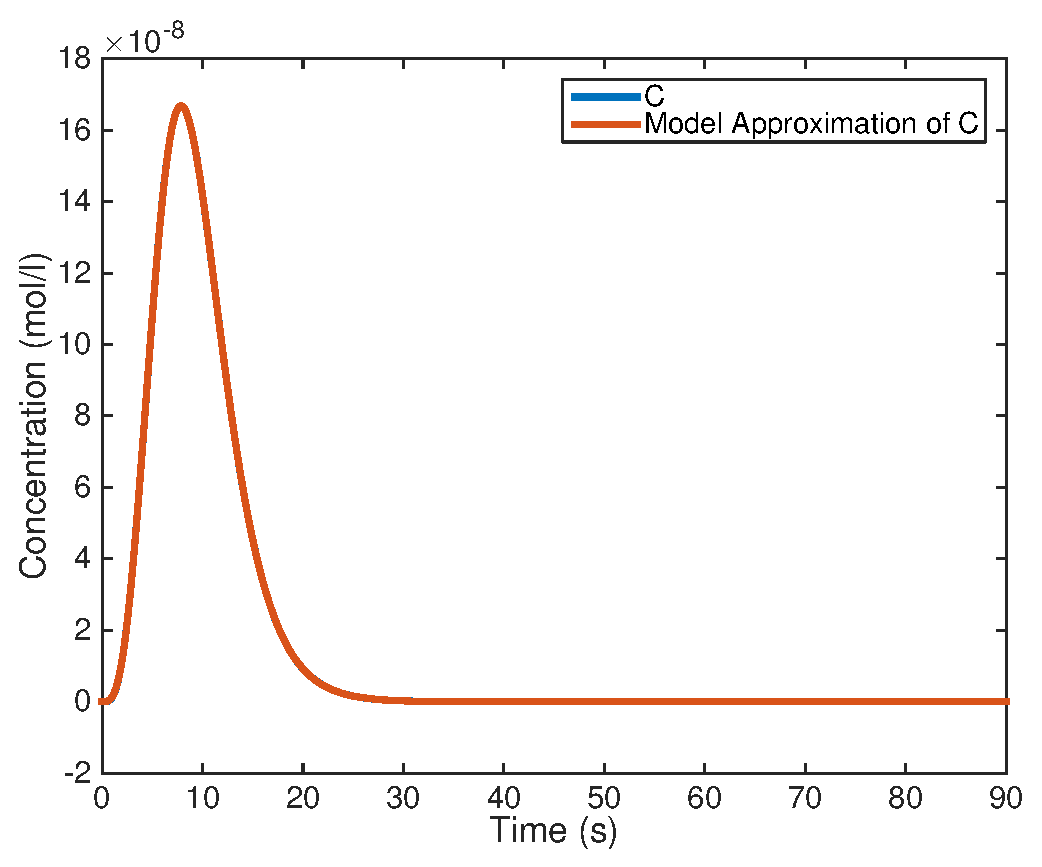
\includegraphics[width = .45\textwidth]{./figs/C-and-Crec.eps} & 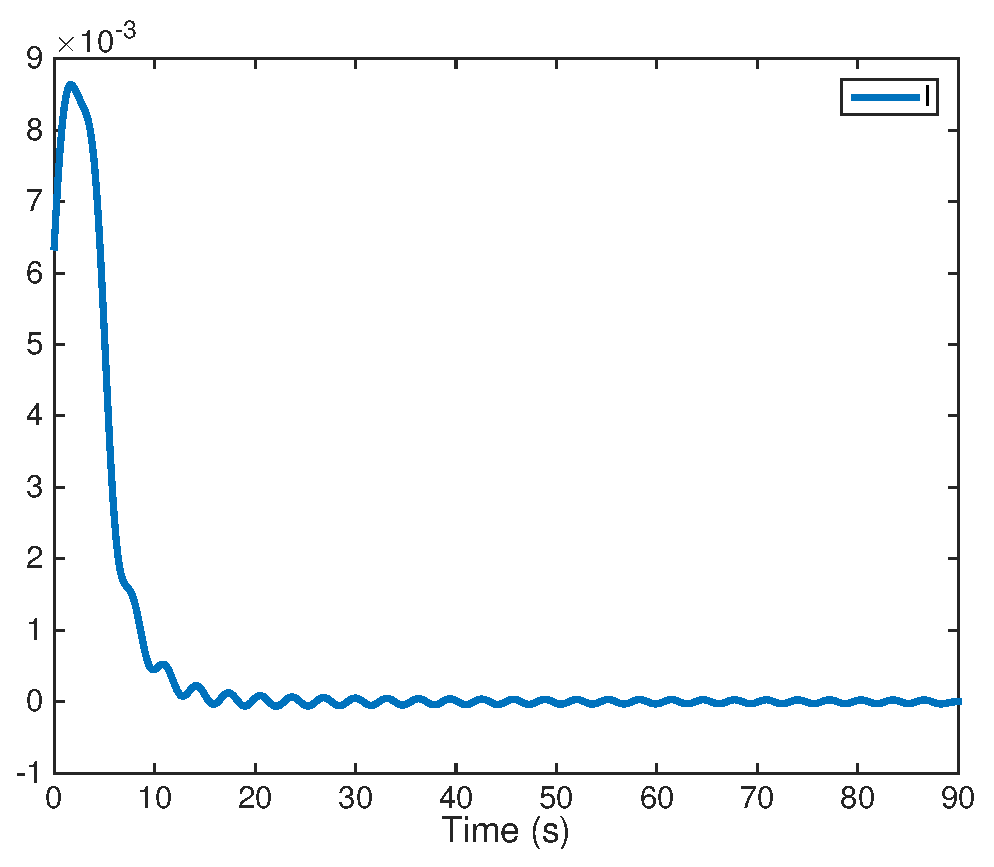
\includegraphics[width = .45\textwidth]{./figs/Irec.eps} \\
				 \multicolumn{2}{ c }{(a) Entire Domain, PMM} \\
				 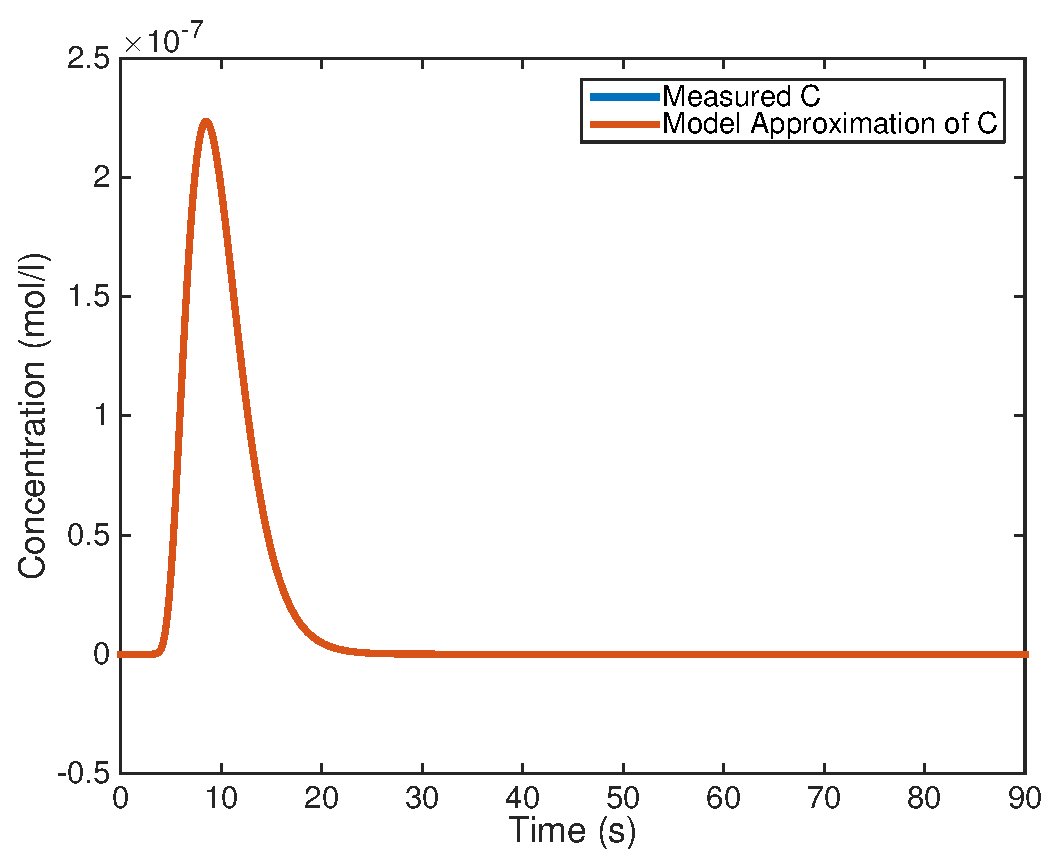
\includegraphics[width = .45\textwidth]{./figs/C-and-Crec-PDE.eps} & 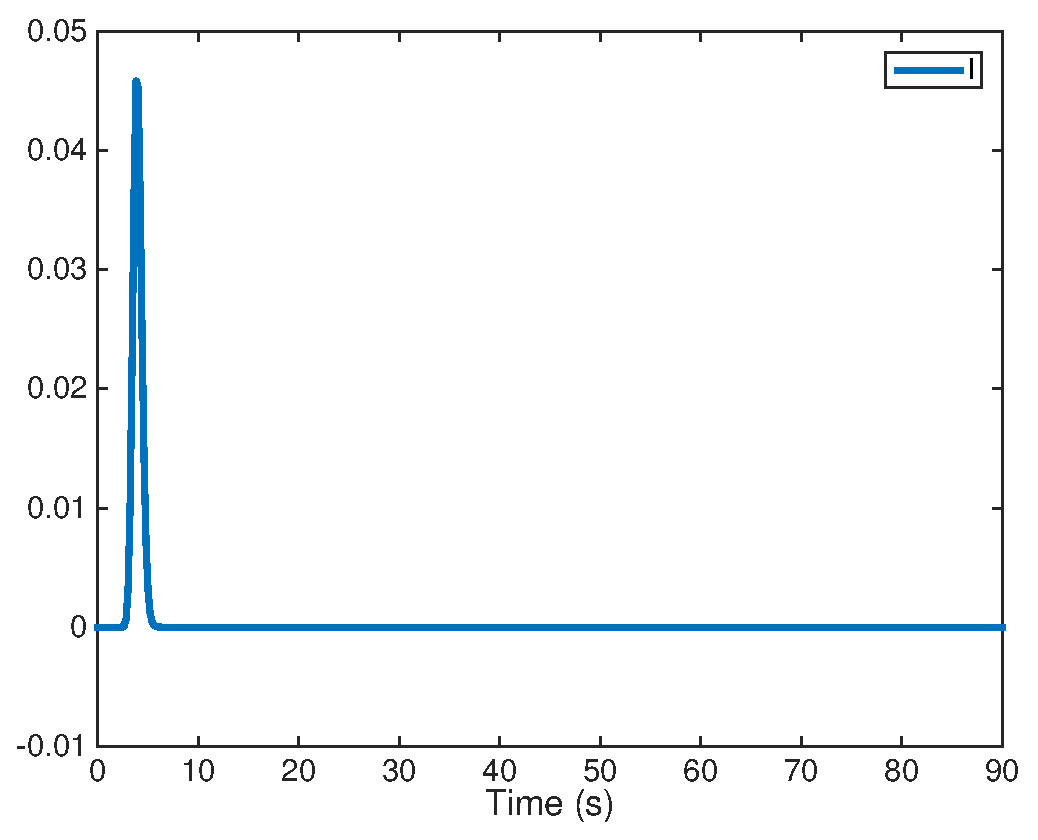
\includegraphics[width = .45\textwidth]{./figs/Irec-PDE.eps} \\			 
				 \multicolumn{2}{ c }{(b) Inside the capillary bed, PMM at $(i,j)=(50,50)$} \\				 
				 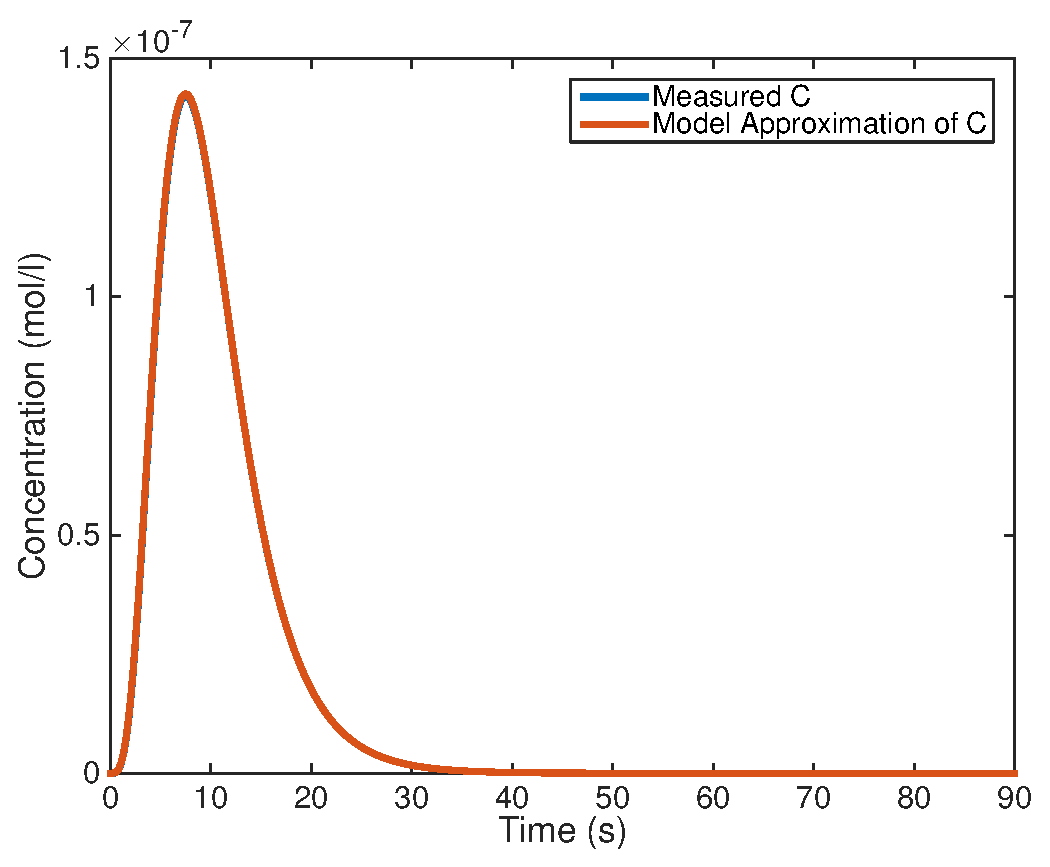
\includegraphics[width = .45\textwidth]{./figs/C-and-Crec-conv.eps} & 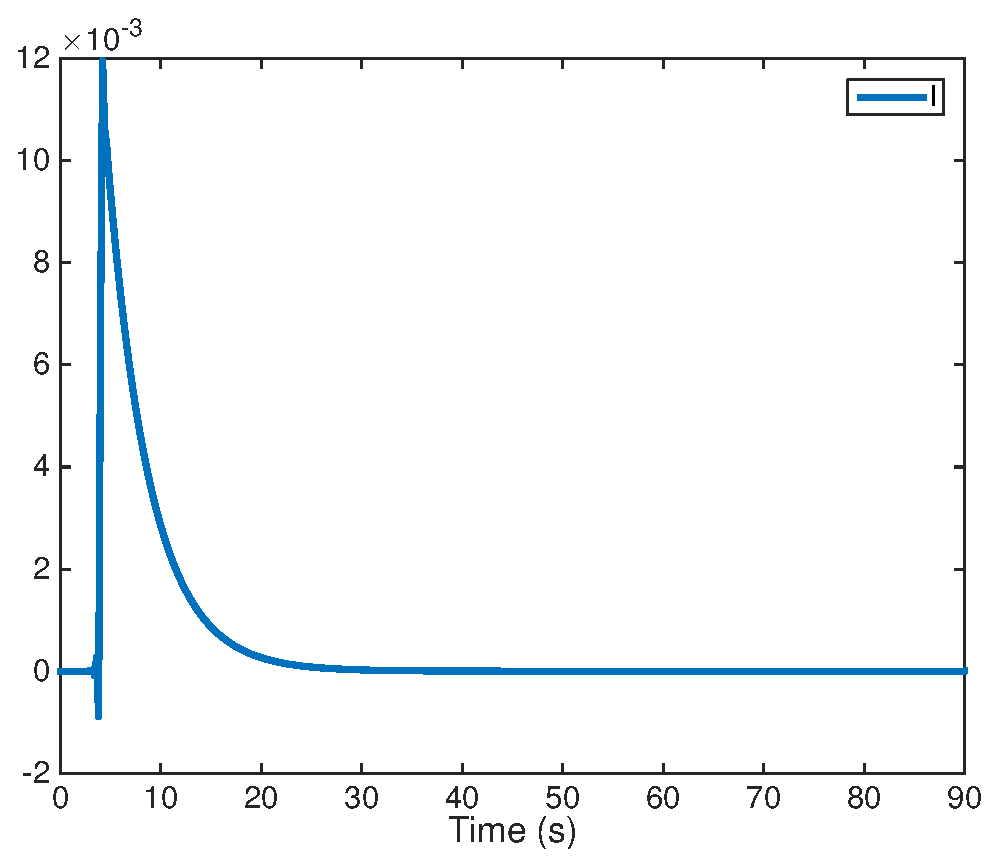
\includegraphics[width = .45\textwidth]{./figs/Irec-conv.eps} \\			 
				 \multicolumn{2}{ c }{(c) Inside the capillary bed, ConvM at $(i,j)=(50,50)$} \\				 				 
			\end{tabular}
		\caption{Results for the deconvolution model. First row: Results of bSVD applied to PMM with block-size (64,64) (i.e. entire domain) (Model-Fit and Impuls-Response Function). Second row: Results of bSVD applied to a single voxel of the PMM in the inside of the domain. Third row: Second row: Results of bSVD applied to a single voxel of the SCD in the inside of the domain. In all cases the model restored the measured concentration curves perfectly.}			
		\label{fig:deconvResults}
	\end{figure}

	
	
	%--------------------------------------------------
	%--------------------------------------------------
	% Section: Discussion
	%--------------------------------------------------
	%--------------------------------------------------	
	\section{Discussion}\label{sec:conclusion}
	Results in Tab. \ref{tab:resultsSim} are indicating good performance of both models to restore the perfusion for an entire volume. 
	Errors are $2.6\%$ for the Maximum-Slope model and $1.3\%$ for the deconvolution model.
	However, the results of the deconvolution model depend on a heuristic choice of the regularization parameter \missingsource.
	Results on a voxel-level are looking quite different (see Tab. \ref{tab:resultsSim}).
	Here the perfusion is grossly overestimated by both the deconvolution model and the the maximum-slope model.
	Errors are in the range of far over $100\%$, indicating a lack of validity of the classic models.
	This impression is supported by the recovered impuls-response functions, displayed in Fig. \ref{fig:deconvResults}.
	Although classic models assume monotonously decreasing residue-functions, the impuls-response functions we obtained are clearly violating this property.
	These effects might be due to dispersion effects \cite{calamante03} and are subject to current investigations.
	
	However, as expected the deconvolution model worked quite good for the ConvM-dataset (see Tab. \ref{tab:resultsSim}). 
	But results are deteriorating if several volumes are averaged, leading to errors of up to $20\%$.
	This can be interpreted that even if the assumptions of the classical models are fulfilled, parameter-estimation will be sensitive with respect to broad resolutions.
	As already described in Sec. \ref{sec:NumExp}, the maximum-slope model fails to restore perfusion correctly due to the assumption of well-mixed compartments.
	Taking into account all of these observations we arrive at the following conclusions:
	If classical models are valid, a too broad spatial resolution might lead to significant errors in the estimation of perfusion parameters.
	On the other hand, a too fine resolution might lead to voxels placed inside of the capillary bed and hence to a dramatic overestimation of CBF.
	A method to determine the appropriate size of voxels is unknown to the authors, as it is coupled to the validity of the assumptions on the models.
	
	Concluding, we have proposed a novel method to validate classical models for perfusion analysis.
	Based on porous media modeling, we described an easily extendable model to simulate CA-flow through a volume of interest.
	The proposed model assumes stationary and linearity of flow as well as spatially constant blood-volume.
	In this form it is completely in line with current pharmacokinetic modeling \cite{sourbron14}.
	In order to connect (medical) volume perfusion with (physical) surface flow, a novel relationship between these two was introduced.
	For the experiments we have confined to a most simple setup, modeling a volume of interest with one inlet, one outlet and constant porosity.
	However, a more sophisticated simulation including more inlets and outlets at spatially varying locations as well as porosity can be set up readily.
	We showed that under these assumptions classical models are yielding good results for perfusion values and can indeed be used with high reliability.
	But as soon as the assumptions are violated, which is the case for the capillary bed, significant errors are introduced.

	Since current validation of deconvolution algorithms is typically performed in the inverse-crime setting, the developed model could be used as an additional reference standard for validation.
	In the proposed modeling, exact perfusion values for the whole tissue can be modeled. 
	Using this method it is hence possible to quantify errors introduced by e.g. different numbers of input and output, more complex flow or even leakage.
	
	As future work we will further investigate the impuls-response functions of the capillary bed and will simulate more complex phenomena in the tissue.

	
	%--------------------------------------------------
	% Bibliography
	%--------------------------------------------------
	\bibliographystyle{ieeetr}	
	\bibliography{./bibliography}

	
\end{document}